%%==================================================
%% chapter03.tex for BIT Master Thesis
%% modified by 朱杰
%%==================================================
\chapter{基于稳定标签传播的非重叠社区发现算法}

由于社交网络“小世界”、“无标度”的特性以及目前社交网络普遍具有大规模的数据量,这对算法的时间复杂度提出了严格的要求。尽管至今已有为数不少的社区发现算法被学者们相继提出,但是这些算法大多是在社区识别的准确率上进行不断创新和优化,针对的多是中小规模的网络,面对大规模的社交网络数据这些算法往往需要巨大的时间开销。而本文在第一章节国内外研究现状中也已经提到,标签传播算法(LPA算法)\cite{Raghavan2007Near}是目前算法时间复杂度最低的社区发现算法,算法简单易理解且不需要任何先验信息,但是标签传播算法也有些许问题,例如稳定性差和算法无法收敛等。
% 截至今天已经有不少学者在LPA算法的基础上进行了改进和创新,例如Leung等人\cite{Leung2009Towards}引入了启发式思想,在节点属性中加上了创新提出的hop score值,以此来提高算法效率及性能;文献\cite{He2014A}则是修改了LPA算法迭代的终止条件;LabelRank算法\cite{Xie2013LabelRank}创新的提出了标签概率矩阵,此法解决了LPA算法运行结果不稳定的问题。

标签传播算法是最早的基于标签传播思想的非重叠社区发现算法,本章节基于该算法进行研究和改进,将提出一种稳定的基于标签传播的非重叠社区发现算法(Community Detection Algorithm Based on Stable Label Propagation),下文简称CDABSLP算法。

CDABSLP算法通过采用异步标签更新的策略来避免LPA算法标签传播过程中可能产生震荡的问题;在节点迭代更新标签时将节点按照节点的重要性降序排列,而非原始的随机顺序;在设计节点重要性评价指标上引进了k-核分解方法,设计了一个全新的综合节点自身影响力以及邻居节点影响力的节点影响力模型;在标签选择方式上同样进行相应的改进,针对出现多个最多邻居标签的情况,在节点影响力模型的基础上设计了标签影响力模型,选取标签影响力最大的标签进行更新。在这一系列改进之后,使得标签传播过程更加稳定,收敛速度快速。

本章接下来的内容组织结构上将先介绍一下标签传播算法的情况,详细分析LPA算法目前存在的缺陷;然后详细的阐述CDABSLP算法在使得标签传播更加稳定性上的设计;接着是对算法整体执行步骤进行全面的说明,并对算法时间复杂度进行分析;最后在验证实验部分中,介绍了包括实验环境、实验数据集以及评价指标后,将会详细的分析在真实网络以及人工基准网络上的实验结果,通过与其他基准算法进行对比实验,以此来证明算法的效果。

\section{标签传播算法的缺陷分析}

标签传播算法早在2002年就被Zhu等人\cite{Zhu2002Learning}提出,这是一种基于图的半监督机器学习算法,它的基本思想是用已经标记的节点的标签信息来预测未标记节点的标签信息。如本文在第一章节国内外研究现状中提及的,是Raghavan等人\cite{Raghavan2007Near}于2007年第一次将LPA算法应用于社区发现领域。LPA算法的主要思想就是利用复杂网络固有的拓扑结构中隐藏的信息来引导探测出网络中存在的“社区”。在起始的时刻,LPA算法会为网络中所有的节点分配一个独一无二的标签,通常就是节点的ID,这代表所有的节点都是单独的一个社区;然后就是不断迭代着更新所有节点的标签,直至收敛,即不再有标签发生改变为止;在每一轮更新标签的过程中,每个节点会将自己的标签修改为自己邻居节点中出现次数最多的那个标签,当出现多个邻居节点的标签均为最大出现数时,随机选择其中一个标签进行更新。在整个重复迭代更新标签的过程中,联系密切的节点最终会被标记为同样的标签,这样在标签传播结束之后,LPA算法可以按照节点不同的标签将节点进行社区划分。

图\ref{fig:dingdianbiaoqianchuanbo}展示了网络中一个节点获取标签的过程。图中的灰色节点在更新其标签时,它拥有的5个邻居节点之中有三个邻居节点标签为为黑色,而两个邻居节点为白色,故将其节点更新为黑色。

\begin{figure}
  \centering
  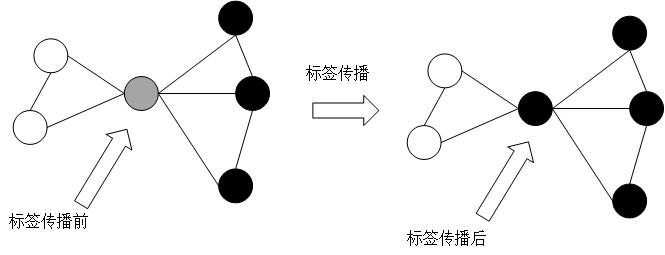
\includegraphics[width=0.75\textwidth]{figures/dingdianbiaoqianchuanbo}
  \caption{节点获取标签的示例图}\label{fig:dingdianbiaoqianchuanbo}
 \end{figure}

公式\ref{eqn:biaoqiangengxin}为标签传播算法中节点更新标签的公式。

\begin{equation}
  \label{eqn:biaoqiangengxin}
  c_i=\arg\max_l \left | \Gamma _i^l \right |
\end{equation}

其中$\Gamma _i^l$表示的是具有标签$l$的节点$i$的邻接节点集合。

标签传播算法执行步骤的具体实现伪代码可参考算法\ref{alg:LPA}。

\begin{algorithm}[htb]  
  \caption{标签传播算法(LPA)}  
  \label{alg:LPA}  
  \begin{algorithmic}[1]  
    \Require
      社交网络$G=(V,E)$,节点总数$N$,最大允许迭代轮数$maxIter$,停止迭代标签修改率$stopIterRatio$;  
    \Ensure  
      网络中所有的社区及其成员;  
    \State  初始化阶段:

    (a)标签初始化:为所有节点设置初始标签,设为其节点ID即可;

    (b)迭代次数初始化:迭代次数$iter = 0$;

    (c)标签改变数初始化:标签改变数量$changedNum = 0$

    \State  标签传播阶段:
      
    (a)如果迭代次数$iter > maxIter$,停止标签传播,转步骤3;否则继续算法;
    
    (b)将网络中的节点按照随机顺序加入待更新标签队列;
    
    (c)针对队列中的每个节点,遍历其邻居节点,选择邻居节点中出现次数最多的标签,将自身标签更新为该标签;若最大出现次数标签存在多个,则随机选择其中一个即可;
    
    $//$注意此处在邻居节点的标签选择上需要说明的是:在第$iter$轮迭代中,无论邻居节点是否已经在本轮迭代中更新过标签,选择的都是邻居节点第$(iter - 1)$轮中的标签;该更新策略称为同步更新;
    
    (d)若节点标签进行了修改,标签改变数量$changedNum + 1$;
    
    (e)每轮标签传播迭代完毕,检查标签修改比例$\frac{changedNum}{N}$;若$\frac{changedNum}{N} < stopIterRatio$,则停止标签传播,转步骤3;反之令$(iter = iter+ 1)$,转步骤2,继续下一轮迭代;
    \State  社区划分阶段:将具有相同标签的节点划分为一个社区,整个网络中存在的标签数量即是发现的社区数量。
  \end{algorithmic}  
\end{algorithm} 

标签传播是通过相邻节点之间标签的传递来实现社区的划分的,其能够实现较好划分效果的原因是:在社交网络这种特殊的结构之中,节点之间通过边相连通,边本身就代表着节点间的联系,那么就不难理解,节点之间相邻这一事件本身就说明着在某种意义上它们是具有某种相似的属性的,这在标签传播中表现即是相邻的节点理应拥有相同的标签;而如果某个节点集合中各节点之间都有着复杂的关联,或者说它们在某种属性上可以被划分到同一类别,那么在网络中的表现也就是存在着大量的边在这些节点之间,在标签传播的结果上这些节点也就应当有着相同的标签,这实质上也就是达到了聚类的效果。概括来说,正是因为社交网络自身的结构特性,它能直观地表现各个实体之间的关联以及实体的分布规律。

LPA算法虽然简洁明了易实现,但是也存在着一些缺陷使得算法实验结果很不稳定。下面进行简单分析:

首先,LPA算法无法保证算法必然收敛。就以算法\ref{alg:LPA}中的提到的最大允许迭代轮数$maxIter$和停止迭代标签修改率$stopIterRatio$而言,这两个参数设置的初衷正是因为LPA算法的不稳定,无法保证算法必然收敛,若不在迭代次数上进行限制,甚至会陷入无限死循环;例如:在含有二分结构的网络之中进行标签传播存在着标签来回更替而进入“死循环”的问题,如图\ref{fig:fig3-1}中所示。

\begin{figure}
  \centering
  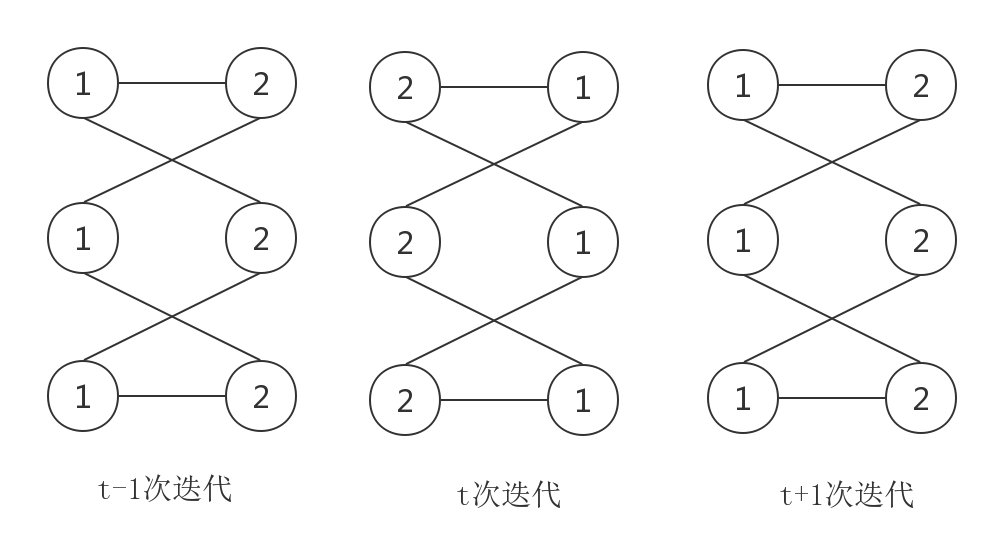
\includegraphics[width=0.75\textwidth]{figures/fig3-1}
  \caption{二分网络中的标签震荡现象}\label{fig:fig3-1}
 \end{figure}

其次,LPA算法第二个不确定性在于其节点更新顺序的随机性。然而很明显的是节点的更新顺序对最终的结果会有很大的影响,且网络之中的不同节点显然是有着不一样的重要程度的。设想一个本来在网络之中起着至关重要作用的节点,如果碰巧被分在最后一个更新标签,那么本轮更新,该节点对其他节点将不会造成任何影响,这显然不是一个很好的选择;即使这对算法的结果没有过多影响,多多少少也会降低算法的收敛速度。最先将重要的节点进行标签更新,显然有助于加快标签的传播。正是在节点更新顺序上的随机性,使得算法存在着不稳定的因素,因此若想要获取稳定的标签传播,在这一方面的改进是必不可少的。

最后,LPA算法第三个不确定性在于其标签选择上随机性。正如算法\ref{alg:LPA}中描述的,当最多出现次数的标签存在多个的时候,随机选择其中一个进行标签更新。很显然当出现多个最大标签时,应该选择的是对自身影响最大的那一个,而不是简简单单的随机选择一个。当然,这就涉及了一个新的问题:对节点之间相互的影响值该如何考量。

经过上述分析可见,原始的LPA算法的确存在着不少有待改进的地方。无论是节点的更新顺序还是在标签的选择方式上,其中的随机性不仅可能影响了算法的收敛速度,甚至可能导致最后的社区发现结果也不稳定。因此,对标签传播算法稳定性问题的解决显得非常必要。下文将提出一种改进的LPA算法以克服原始LPA算法的不足。

\section{算法核心思想}

\subsection{异步更新标签}

在上一小节中提及了LPA算法实验结果不稳定,准确率较低,尤其是算法收敛速度不稳定,甚至可能无法收敛。而这与其标签更新时采用的同步更新策略有关,这在算法\ref{alg:LPA}中也有提及。为了更好的对比突出异步更新标签的优势,下面先介绍一下同步更新与异步更新的概念。

因为每个节点不可能同时更新它们的节点标签,所以在整个网络之中所有节点在更新标签的时候必然存在着先后顺序。在某个节点更新标签的时候,它的部分邻居节点可能已经在它之前进行过标签更新了,而也有部分邻居节点仍然未更新标签,这样一来在标签选择上就面临了一个问题:对于已经在本轮迭代中更新过标签的邻居节点,该节点是选择最新的标签进行参考还是依旧选择上一轮结果中标签。

标签的同步更新是指在每一轮标签传播过程之中,某个节点在考察其邻居节点标签以更新自身标签的时候,无论邻居节点是否已经经历过本轮迭代,均参考的是邻居节点上一轮标签迭代后的结果;而标签的异步更新则参考的是已知最新的邻居节点标签,即:若邻居节点已经经历过本轮迭代,就参考邻居节点本轮标签更新后的结果,反之则参考邻居节点上一轮的迭代结果。

如图\ref{fig:tongbugengxinshili}中所示,按照节点ID号$\{1,3,5,6,4,2,8,7 \} $的顺序对图中网络进行一轮同步更新,因为同步更新需要上一轮迭代的结果,故无法直接覆盖原标签结果,因此在图中更新后的标签标记在相应节点的外侧。从整个更新过程可见得到的结果依然十分随机,结果甚至很难收敛。并且在具体划分的过程之中,因为同步更新参考的邻居节点标签均为上一轮迭代的结果,因此其实节点的更新顺序在此也显得无所谓。

\begin{figure}
  \centering
  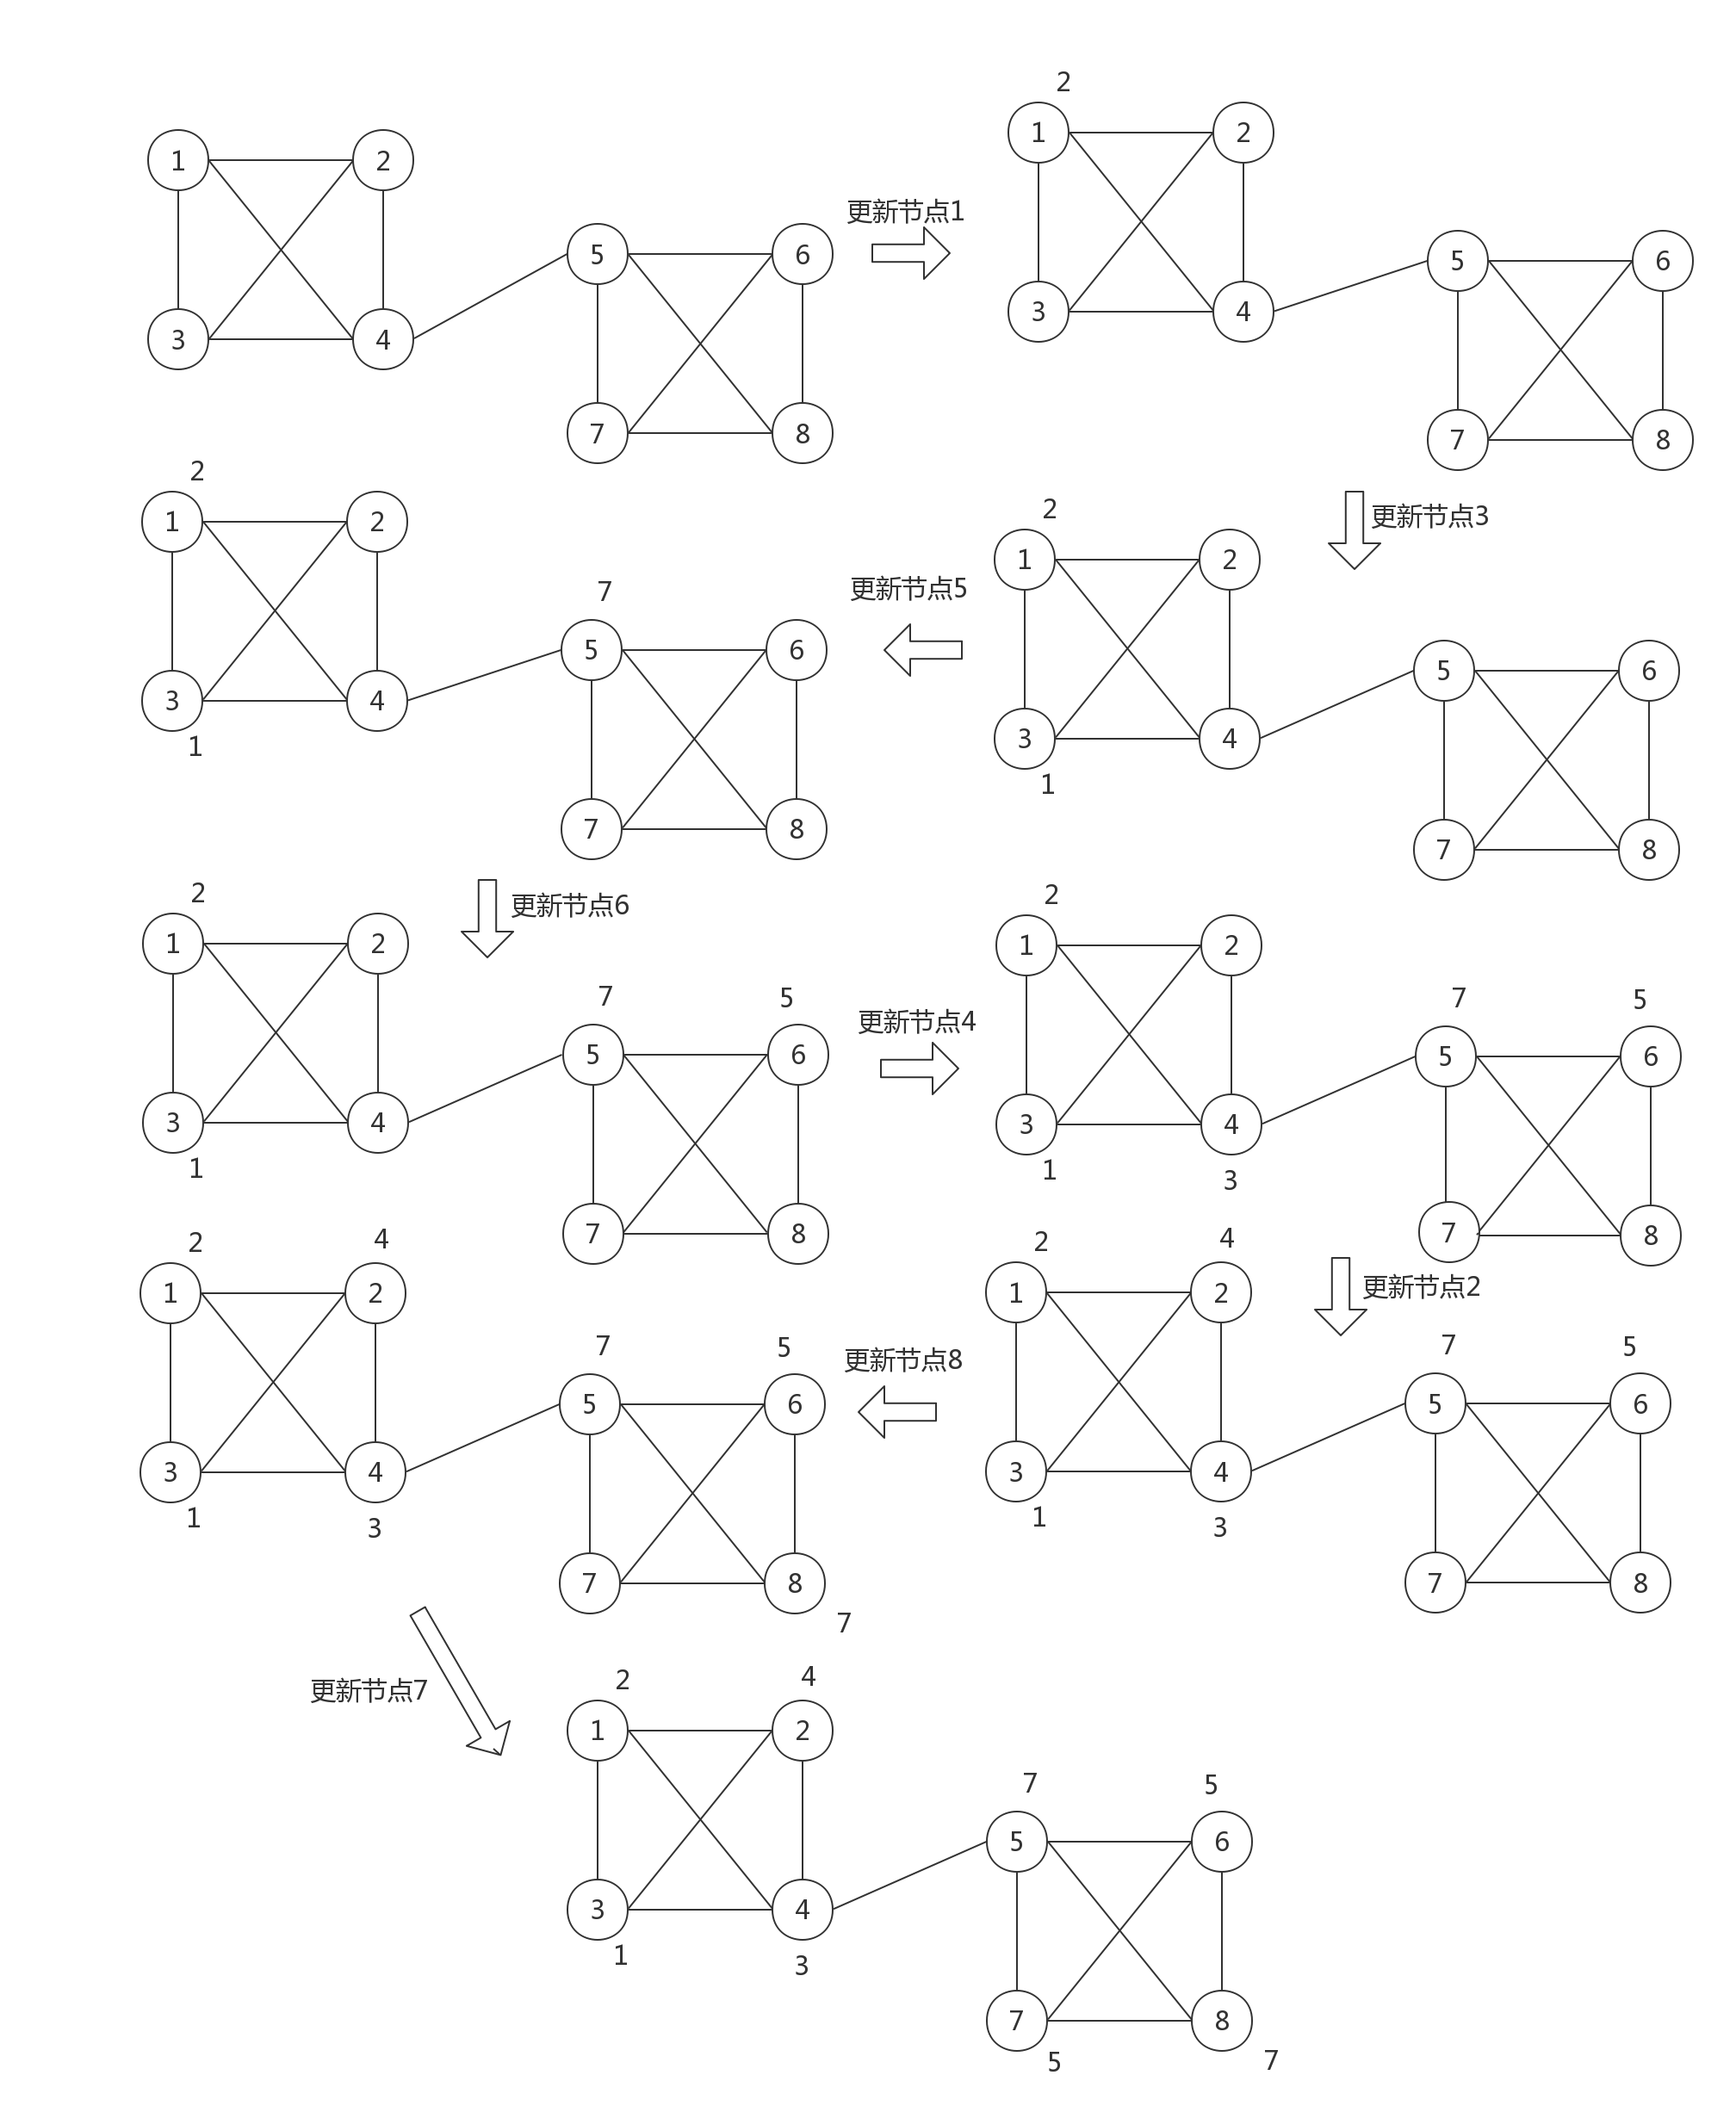
\includegraphics[width=0.95\textwidth]{figures/tongbugengxinshili}
  \caption{标签同步更新示例图}\label{fig:tongbugengxinshili}
\end{figure}

而异步更新则不同,如图\ref{fig:yibugengxinshili}中所示,在示例中按照节点ID号$\{1,3,5,6,4,2,8,7 \} $的顺序对原图中网络进行一轮异步更新,因为无需保存上一轮迭代的结果,故在节点更新标签的时候直接覆盖原标签即可。同样从整个更新过程可见异步的更新过程结果相当令人满意,几乎已经收敛,仅仅只用再多一次迭代就可以获得完整的社区划分。目前标签为“4”的节点在下一轮迭代中也必将被更新为“7”。其他节点均已经在这一轮迭代中被划分到了相应的社区。相比同步更新,显然异步更新的方式更加优秀,不仅能够使得实验结果更加稳定,而且有效地加速了算法的收敛速度。

但是异步更新标签也会对节点的更新顺序以及标签的选择方式提出更高的要求,下面将会介绍本章提出算法在对节点的更新顺序以及标签的选择方式上的改进。

\begin{figure}
  \centering
  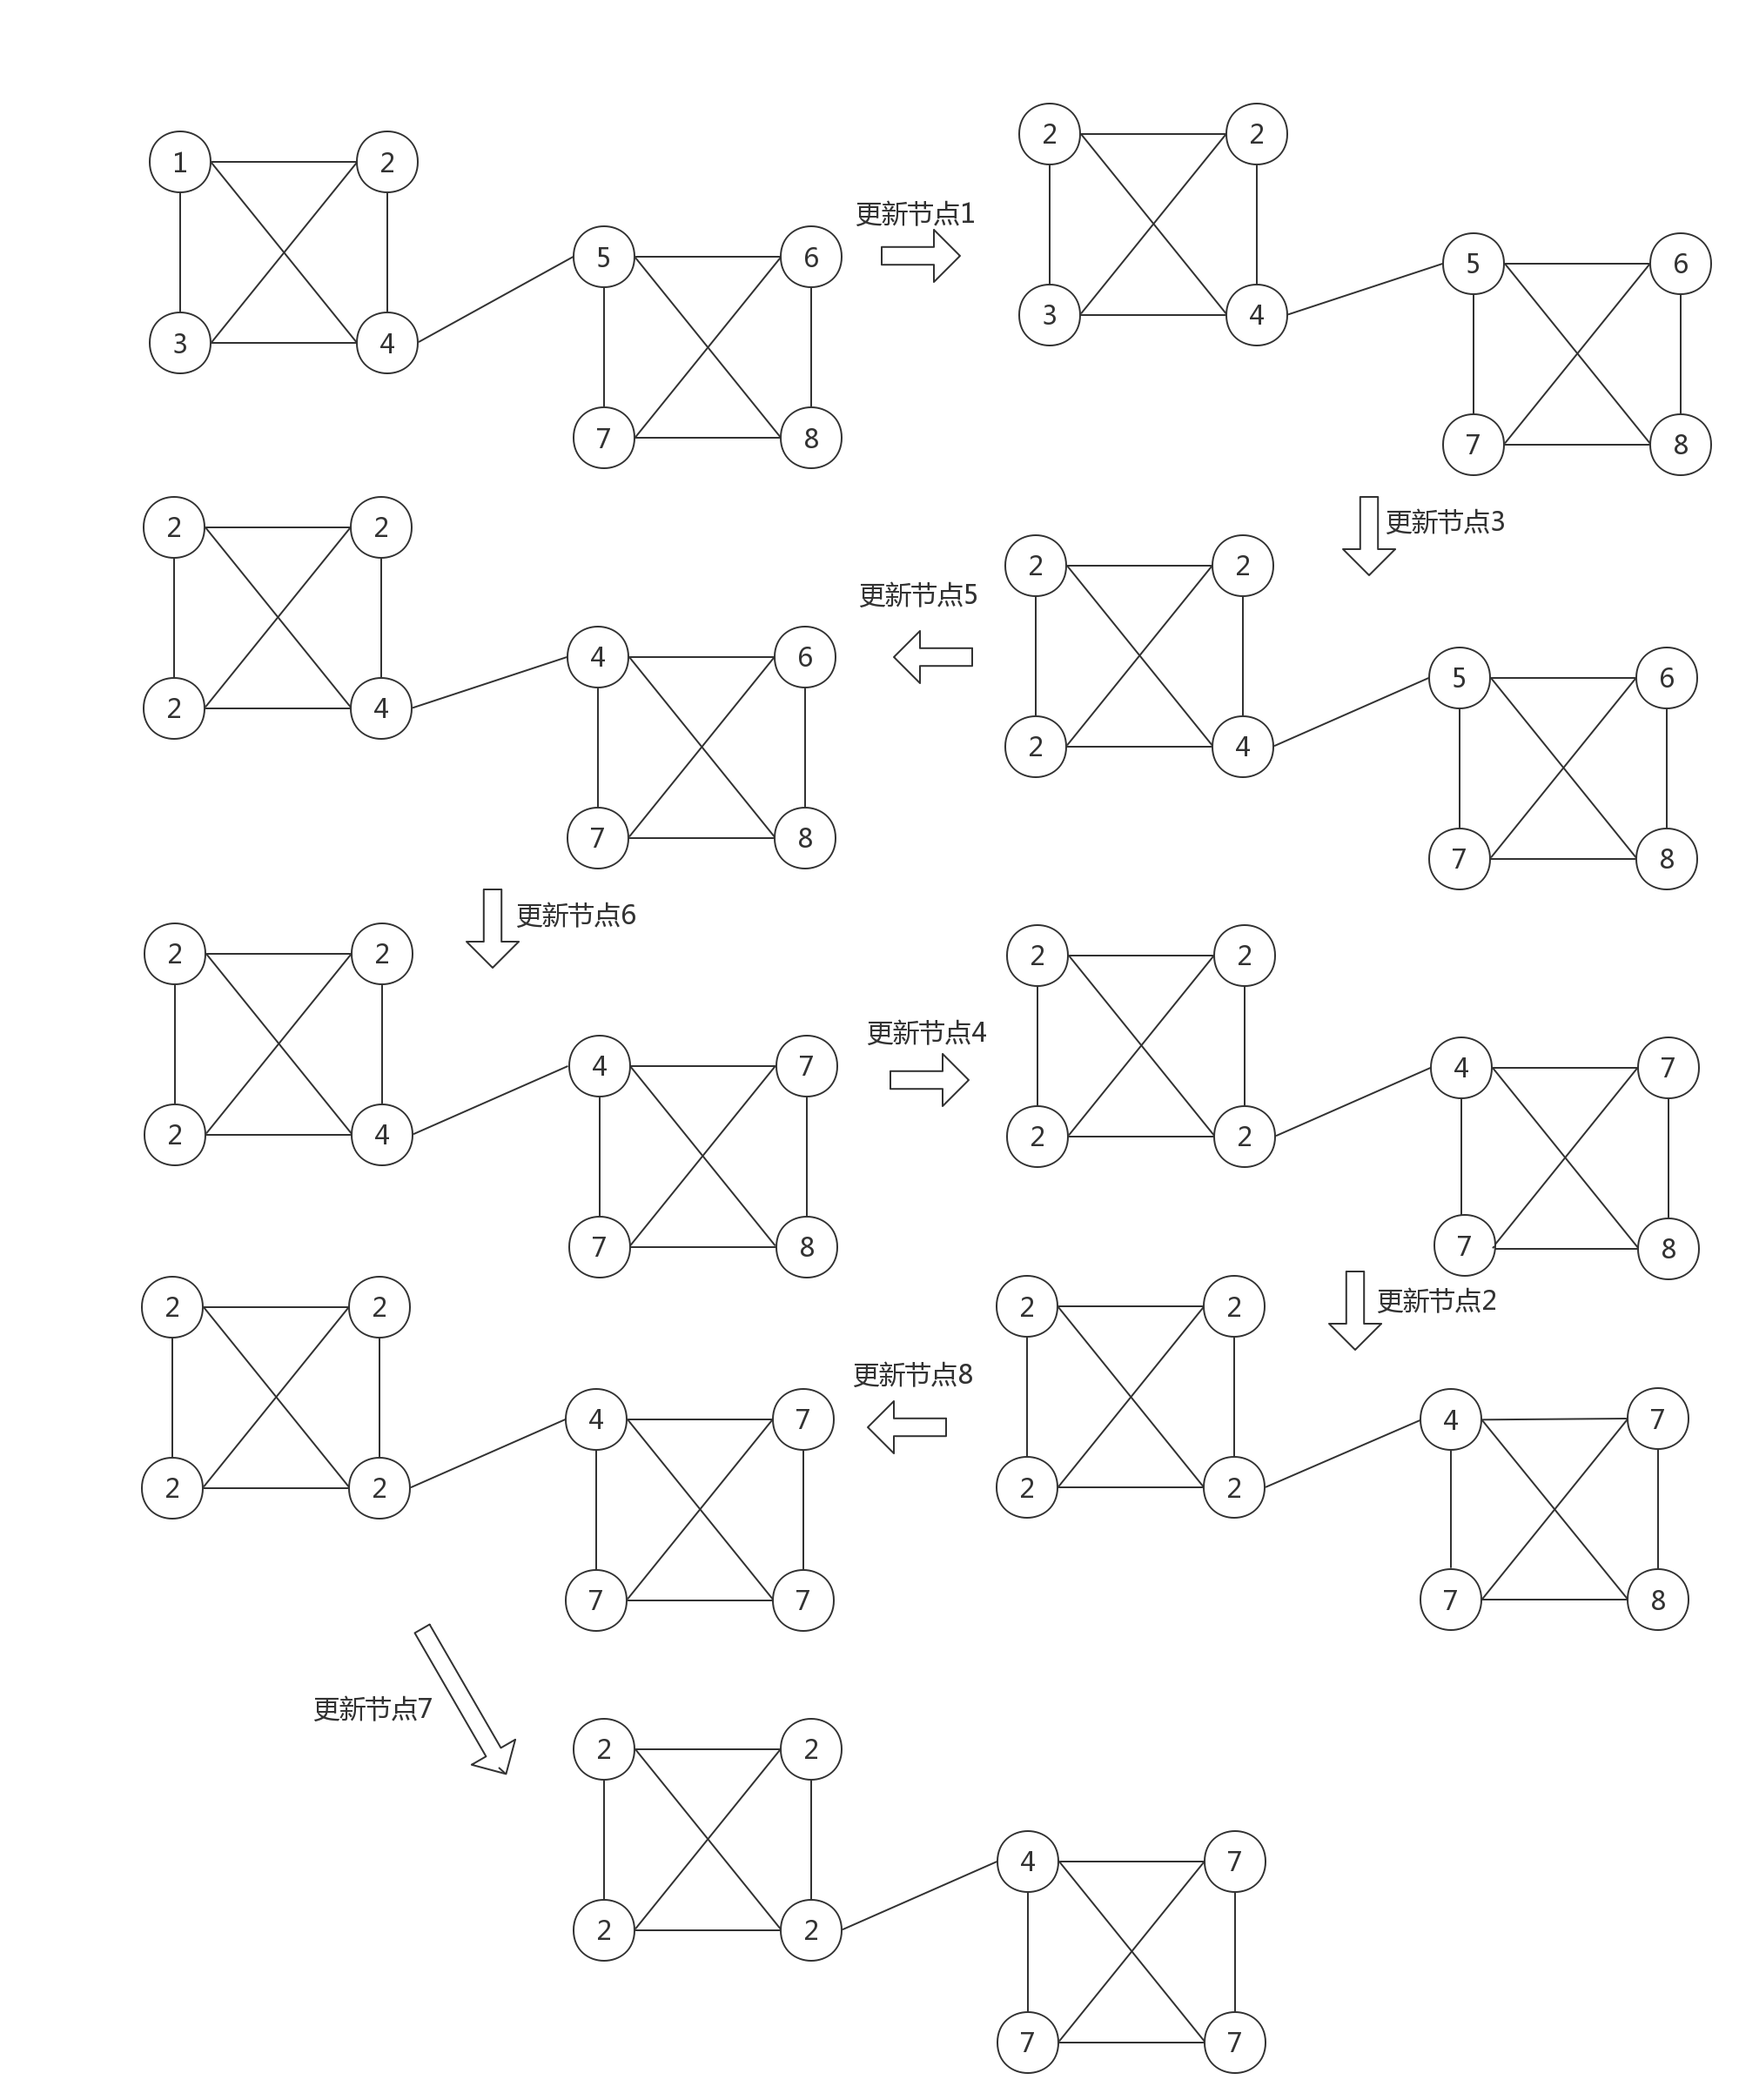
\includegraphics[width=0.95\textwidth]{figures/yibugengxinshili}
  \caption{标签异步更新示例图}\label{fig:yibugengxinshili}
\end{figure}

\subsection{节点更新顺序上的改进}

在采用了异步的标签更新策略之后,虽然使得标签传播更加稳定,也有效地加速了迭代收敛速度,但是异步更新同时也对迭代过程中的节点顺序提出了很高的要求。因为异步更新的缘故,率先进行更新的节点的标签会持续对后续即将更新的节点造成影响,所以如果是社交网络中本就是有着较为重要地位的节点率先进行更新,而社交网络边缘的那些无关紧要的节点最后更新,迭代过程收敛的速度会更快,且最终得到的社区划分也将更为合理。

以一个简洁的网络结构中的异步标签传播过程为例,这是一个5个节点构成的简单网络,如图\ref{fig:jiediansuijigengxinshunxu}中左上角所示。在进行标签传播的过程之中,若按照随机节点顺序进行标签更新,不妨假设按照节点ID号$\{2,1,3,5,4 \} $的顺序进行第一轮标签传播,则可见原始的2号节点率先将其标签更新为它唯一邻居1号节点的标签“1”,然后1号节点自身随机选择了众邻居节点中的一个标签“3”进行了标签更新,最终后续的节点$\{3,5,4 \} $都更新为了标签“3”。这一轮迭代中除了一个节点,其他节点均更新为了统一的标签。在下一轮迭代中,无论如何,标签“1”也会被更新为“3”,最终达到收敛。

\begin{figure}
  \centering
  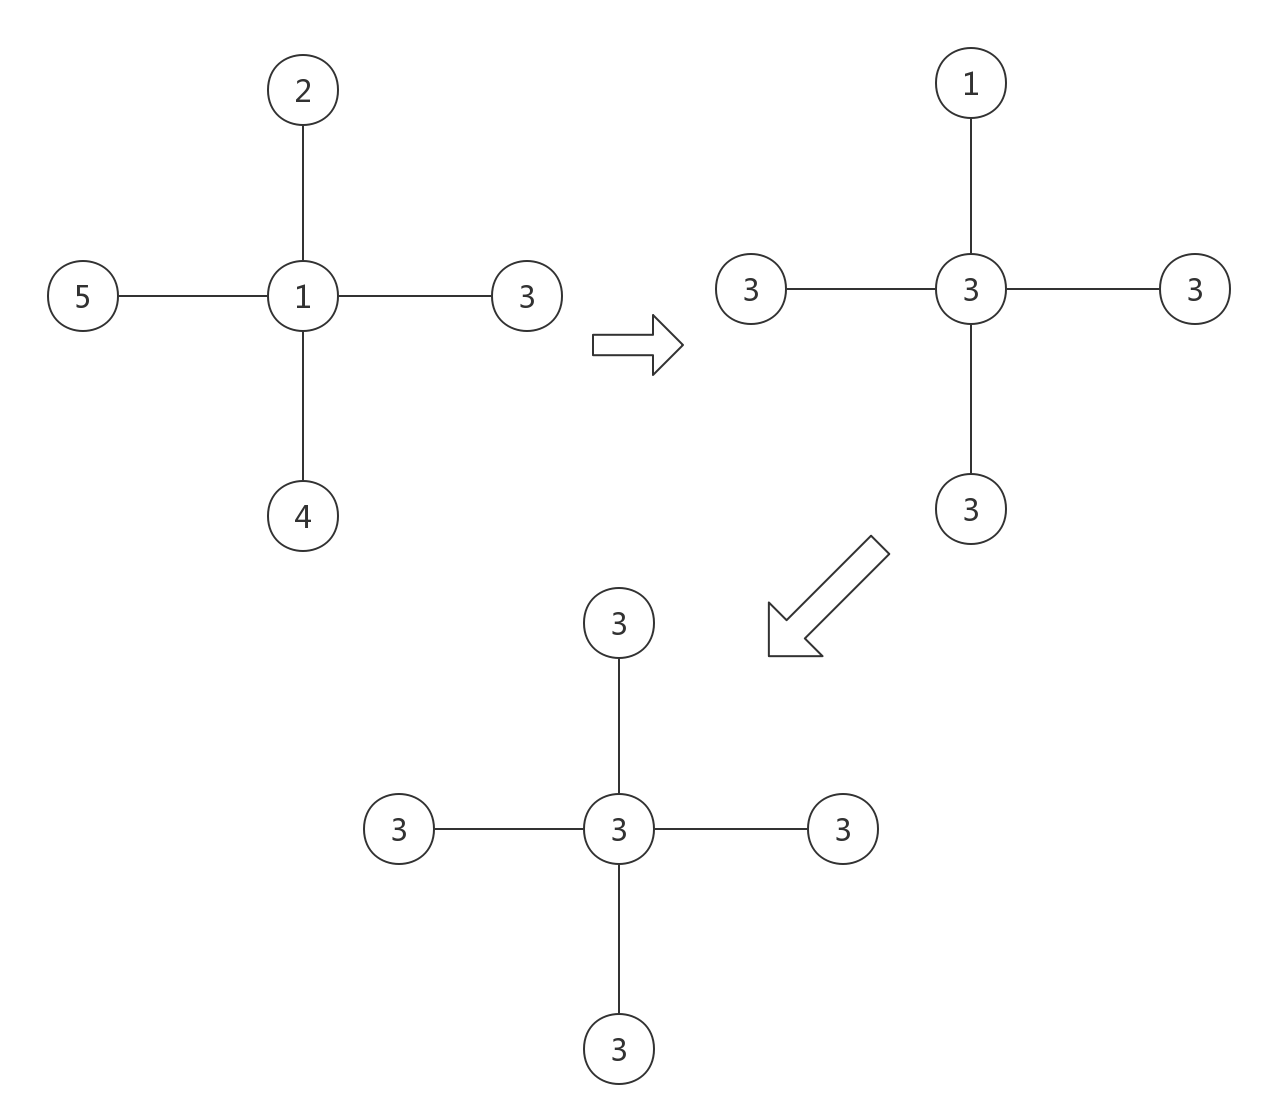
\includegraphics[width=0.75\textwidth]{figures/jiediansuijigengxinshunxu}
  \caption{节点以随机顺序更新的示例图}\label{fig:jiediansuijigengxinshunxu}
\end{figure}

然而在图\ref{fig:jiediansuijigengxinshunxu}中的网络中,很直观地即可看出节点ID号$\{2,3,4 \} $的节点均围绕着1号节点,显然1号节点在这个简单网络结构中具有最重要的地位以及影响度,起着“桥梁”和“枢纽”的作用。如果在节点更新时按照节点的重要性排序来进行更新,那么可想而知那些关键的节点率先更新标签后,可以持续不断地对其他节点的标签更新造成影响。图\ref{fig:jiedianyingxiangzhigengxinshunxu}展示了上述网络中以节点重要性降序排列来进行标签更新的情况。将最重要的1号中心节点率先进行标签更新,而此后其周围节点都会把标签更新为中心节点的标签,在这种情况下仅仅只用了一轮标签迭代后算法就收敛了,相比随机顺序更新少了一轮迭代。而这还仅仅只是在这个简单的示例之中,试想如果是巨大的社交网络,如果按照节点重要性进行排序后再执行标签更新,那么必然会显著地提高算法的收敛速度。

\begin{figure}
  \centering
  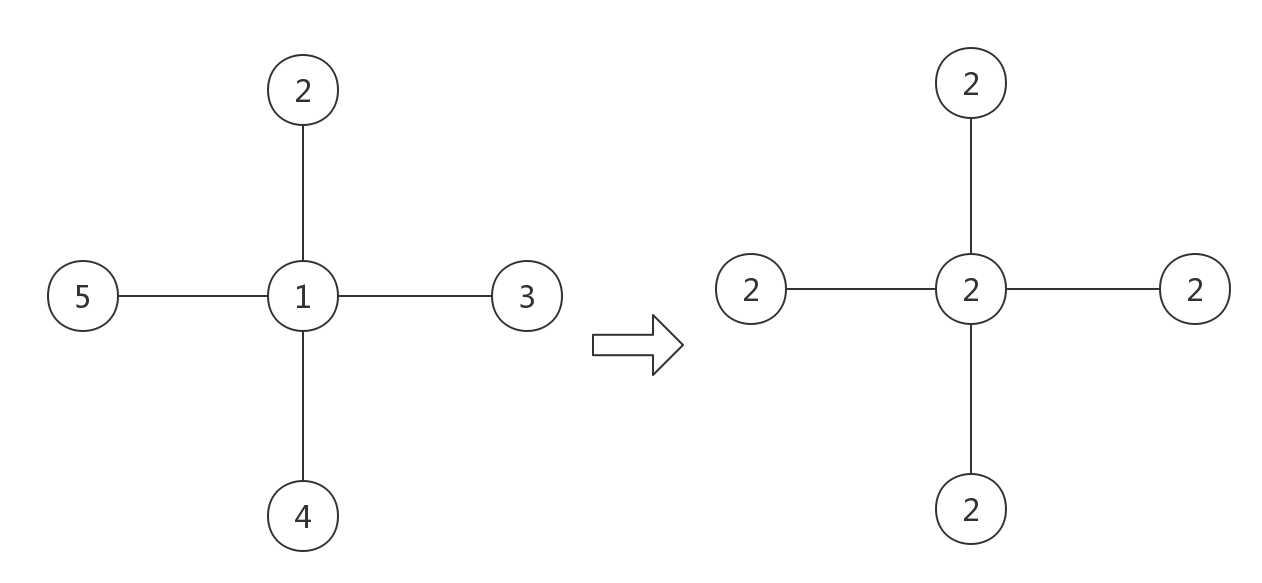
\includegraphics[width=0.75\textwidth]{figures/jiedianyingxiangzhigengxinshunxu}
  \caption{节点以重要性降序更新的示例图}\label{fig:jiedianyingxiangzhigengxinshunxu}
\end{figure}

通过上述分析,本章提出的改进算法将会在第一轮的标签传播之前,先将节点按照节点重要性进行排序,然后在后续的标签传播过程之中,所有的节点按照节点重要性的降序依次更新标签。当然这就涉及了一个新问题,即:如何对节点的重要性进行评判。这一问题的解决方案将会在下一小节中进行详细介绍。

\subsection{节点影响力模型}

在本文第二章研究基础第一小节社交网络的统计特性中,已经提及了多种考量节点重要性或者影响力的统计指标,比如节点的度、聚集系数和介数等等。在这之中,节点的度以及聚类系数虽然均能反应节点在社交网络之中的关键程度,尤其是节点的度因为容易理解且计算方便,不少基于标签传播的改进算法往往会将标签更新顺序直接设置为节点度大小的降序,这样已经能够取得相较原始LPA算法更为出色的效果;但是这两个指标更侧重于社交网络的局部信息,若想要在网络的整体布局上来分析节点的影响力,介数会是一个很好的衡量指标,然而统计网络中所有节点之间的最短路径会消耗巨大的时间,很明显若要对所有节点进行介数的计算,标签传播这一方法仅仅线性时间的执行速度优势将完全不复存在。

而Kitsak等人在文献\cite{Kitsak2010Identification}中提出的k-core分解方法将能很好地解决上述问题,作为一个节点影响力指标。Kitsak等人指出:k-core值高的节点在复杂网络之中具有更强的信息传播能力,即节点的k-core值越高,其影响力越大。

k-核分解方法的核心思路是将整个网络划分为互不相交的多个子网络,在每个子网络中的所有节点在该子网络中的度最小为k。每个节点均有一个k-核值,该值的大小揭示了节点在整个网络中的地位是处在中心位置还是边缘地带,通常可记为$Ks(i)$,表示节点i属于第k-核,但并不属于(k+1)-核。

k-核分解方法的时间复杂度同样只要线性时间,其复杂度为 $O(m)$,$m$为网络中边的总数。通过k-核分解可以分析获取复杂网络的层次性,图\ref{fig:kcoreshili}展示了一个k-核分解的示例,该网络被分解为了三层,此结构就像一个洋葱一样,因此可以很好地反应出网络中的层次性。k-核分解的具体执行步骤可参考算法\ref{alg:k-core},而流程图\ref{fig:k-core}展示了k-核分解法的整个过程。

\begin{algorithm}[h]  
  \caption{k-核分解方法}  
  \label{alg:k-core} 
  \begin{algorithmic}[1]  
    \Require  
      复杂网络$G=(V,E)$;  
    \Ensure  
      k-核划分结果;  
    \State 初始化 $k=0$;  
    \Repeat  
      \State $k = k+1$;
      \Repeat 
        \State 将网络中度小于等于k的节点划分至k-core子集,并删除这些节点以及与这些节点相连的边;
      \Until{网络中不存在度小于等于k的节点}
    \Until{网络中所有节点均已划分完毕}  
  \end{algorithmic}  
\end{algorithm}  

\begin{figure}
  \centering
  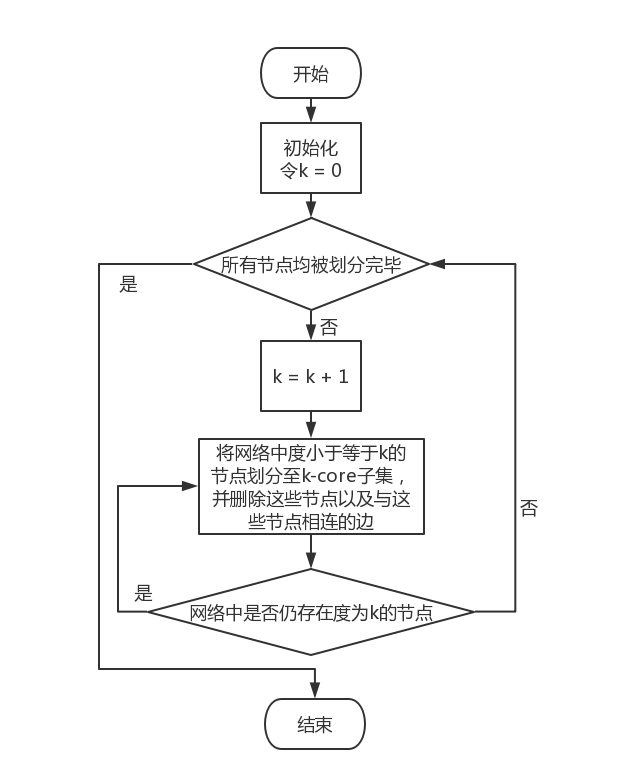
\includegraphics[width=0.75\textwidth]{figures/k-core}
  \caption{k-核分解方法的流程图}\label{fig:k-core}

  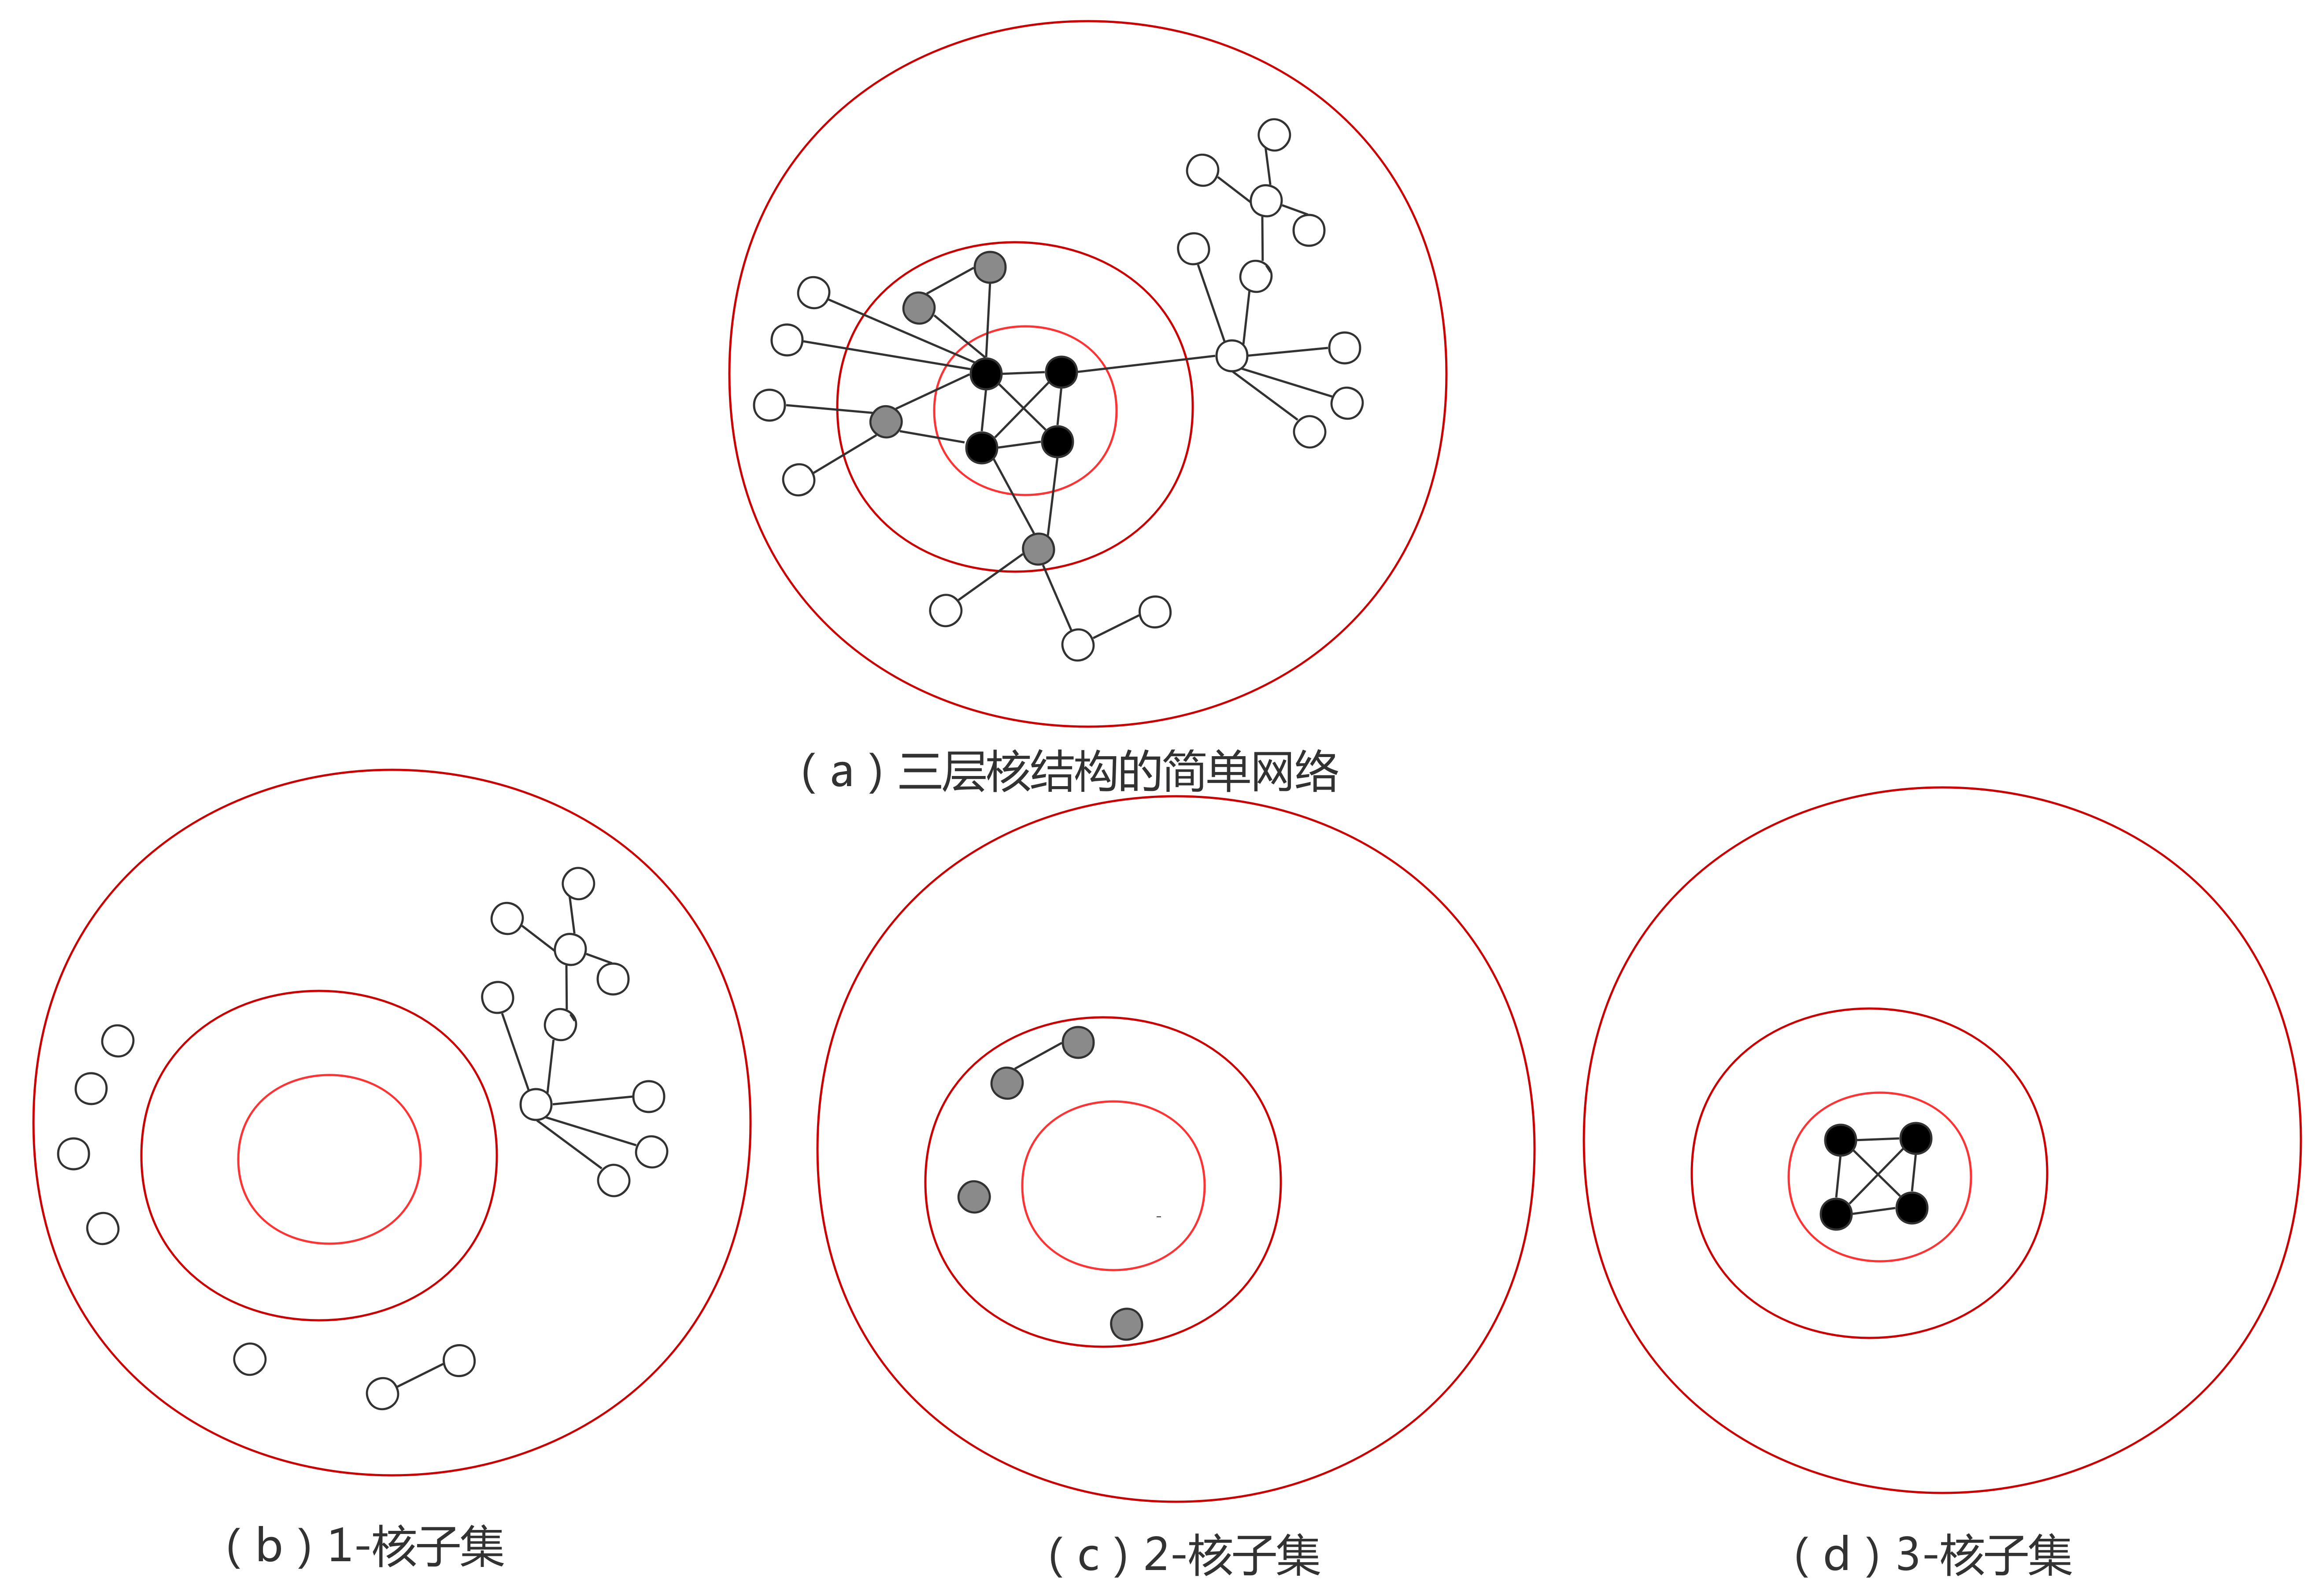
\includegraphics[width=0.75\textwidth]{figures/kcoreshili}
  \caption{k-核分解示意图}\label{fig:kcoreshili}
\end{figure}

节点的k-核值越大,表示它在网络中的位置越是中心,但是在复杂的社交网络之中,仍然存在大量具有相似k-核值的节点会随机的进行排序,因此仅仅依靠k-核值可能还无法较好的对节点进行排列。考虑到节点自身的影响力同样也受其邻居节点影响力的影响,某一节点若与其他关键节点均有连接,则可以认为此节点同样具有较大的影响力。

由此出发,本章提出了一种全新的节点影响力模型--NI(即Node Influence)。该模型在关注节点自身k-核值的同时,也考虑到了节点邻居的k-核值。节点i的影响力$NI(i)$的计算方式可参考公式\ref{eqn:NI}。

\begin{equation}
  \label{eqn:NI}
  NI(i)=Ks(i)+\alpha \cdot \sum_{j \in \Gamma _i} \frac{Ks(j)}{d_j}
\end{equation}

其中,$Ks(i)$上文已经提及,是节点i的k-核值;$\alpha$是用来调节邻居节点影响力的作用大小的可调参数,$\alpha \in [0,1]$;$\Gamma _i$表示的是节点i的邻居节点集合;$d_j$表示的是节点j的度。

按照节点影响力模型计算所有节点的NI值,把所有节点按照其NI值的大小降序排列,在每一轮标签迭代过程中就参照这一顺序进行节点标签更新,这样可以使得算法更加稳定,不再有随机性。

\subsection{标签选择方式上的改进}

在原始LPA算法中还有一大不稳定之处便是其标签选择方式,若一个节点更新标签的时候存在多个出现次数最多的邻居节点标签,原始LPA算法会随机选择其中一个。参考节点影响力模型的设计,本章提出算法在标签更新的时候也引进了节点影响力指标。

若节点i更新标签的时候,邻居节点中存在多个最多出现标签,则依次计算这些标签对节点i的影响力,最终选择影响力最大的标签进行更新;而在节点i更新标签,而邻居节点中存在唯一的最多出现标签的情况下,出于维持低时间复杂度的考虑,依然维持原始算法中的标签选择方式,直接更新节点标签为最多出现标签即可,不再进行无谓的标签影响力计算。此外,当发生极少可能的情况,即在进行了标签影响力计算之后,依旧无法确定采用哪个标签进行更新时,选择保留原标签,不进行任何更新。

公式\ref{eqn:LI}展示了标签$l$对节点i的影响力$LI(i,l)$的具体计算方式。

\begin{equation}
  \label{eqn:LI}
  LI(i,l)=\sum_{j \in \Gamma _i ^l} \frac{NI(j)}{d_j}
\end{equation}

在公式中,$\Gamma _i ^l$表示的是节点i的邻居节点中标签为$l$的节点集合。

% 此外,在标签选择方式上还值得一提的改进是:本章提出的算法在进行标签选择的时候,不仅仅会考虑邻居节点的标签,也会将自身的标签考虑在内。这同样也符合逻辑,以图\ref{fig:biaoqianbugenggai}为例进行分析,图中(a)为原始网络,对该网络进行标签传播时,显然所有节点均为1-核,而因为1号节点

% 而以公式\ref{eqn:LI}为基础的节点标签选择方式可参考公式\ref{eqn:ci}。
% \begin{equation}
%   \label{eqn:ci}
%   c_i=\arg\max_{l \in lmax} LI(i,l)
% \end{equation}

% 异步标签传播策略能够避免标签震荡现象,并且相对同步标签更新策略需要
% 更少的迭代次数,因此这里采用异步标签更新方法。然而由于节点并不是同时更
% 新的,因此节点更新的顺序对社区发现结果的稳定性及社区质量有很大的影响;
% 除此之外,标签传播过程中的标签选择策略也存在不稳定因素,当返回多个标签
% 同时被最大个数邻接点拥有时,LPA 算法随机的选择其中的一个标签作为该节点
% 的新标签,这也造成了 LPA 算法的不稳定性。而 下一章节要提到的COPRA 中也同样存在这些不稳
% 定因素。

% 在简单网络上分析传统标签传播算法的社区发现过程,如图\ref{fig:fig3-2}所示。在
% 该网络中有两个社区,分别是${v_1,v_2,v_3}$和${v_4,v_5,v_6}$。节点上的数字表示该节点
% 的社区标签,初始的时候各个节点的社区标签各不相同,如图\ref{fig:fig3-2}(a)所示。假设
% 经过几次标签传播之后,节点拥有相同的标签“2”,而节点 $v_4$、$v_5$和 $v_6$
% 的标签仍然各不相同,如图\ref{fig:fig3-2}(b)所示。如果首先更新节点 $v_4$
% 的标签,由于它的所有邻接点的标签都各不相同,随机选择标签“2”作为节点 $v_4$
% 的新标签,
% 更新结果如图\ref{fig:fig3-2}(c)所示;然后更新节点 $v_6$
% 的标签为标签“2”,此时节点 $v_5$
% 的两个邻接点的标签都为“2”,它也更新为标签“2”。这样更新后所有的节点都划分
% 到了同一个社区中,这样的社区划分结果没有意义。相反,在更新节点 $v_4$
% 的标签时,如果随机选择的更新标签是标签“6”,如图 \ref{fig:fig3-2}(d)所示;紧接着更新节点$v_5$
% 的标签,根据标签计算公式得到节点 $v_5$
% 的新标签为标签“6”;此时节点 $v_6$的
% 两个邻接点的标签都为“6”,它的标签保持不变。通过这样的标签更新顺序和标
% 签选择方式,能够得到正确的社区划分结果。
% \begin{figure}
%   \centering
%   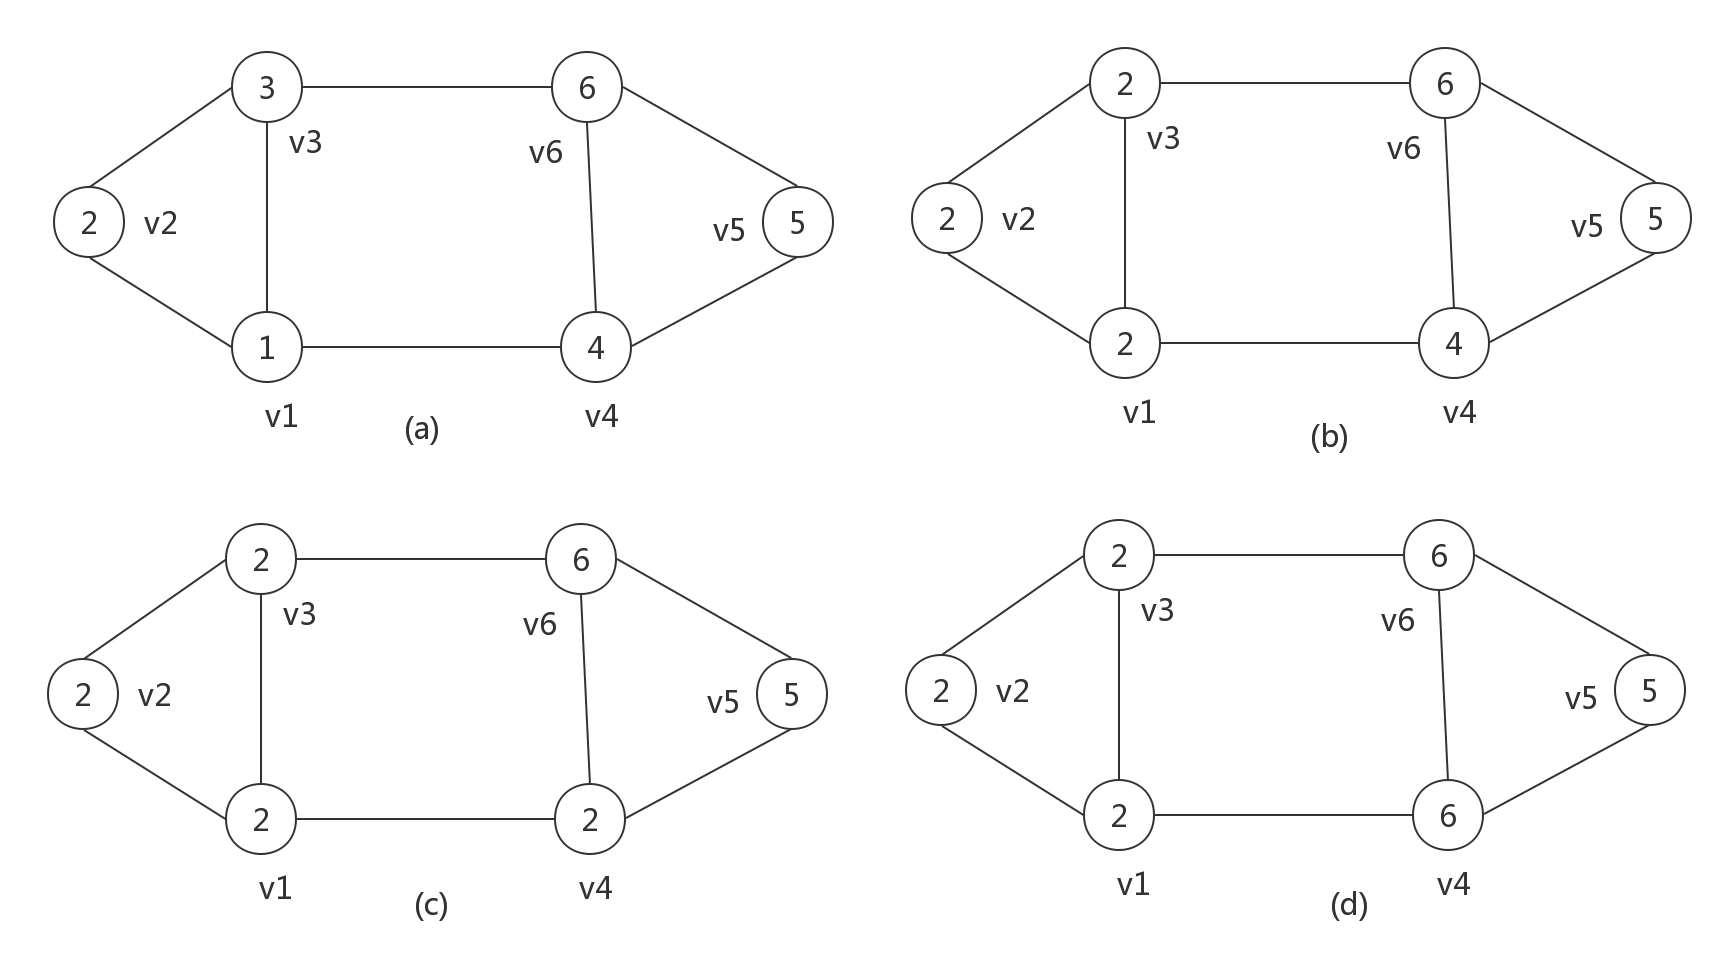
\includegraphics[width=0.75\textwidth]{figures/fig3-2}
%   \caption{标签传播过程示意图}\label{fig:fig3-2}
% \end{figure}

% \subsection{标签选择阶段的改进}
% 造成标签传播算法不稳定的另一个因素是标签选择的机制,当更新一个节点
% 的标签时,如果返回多个标签同时被最大个数的邻接点拥有时,传统的标签传播
% 算法会随机的从中选择一个标签赋给该节点,因此,算法迭代过程很难得到一个
% 稳定的收敛状态。为了提高算法的稳定性,当返回多个标签时,将节点影响值引
% 入到标签更新公式中,选择标签影响强度最大的标签赋给该节点。 

% 标签l对节点i的影响强度计算如公式\ref{eqn:LI}所示。
% \begin{equation}
%   \label{eqn:LI}
%   NI(i,l)=\sum_{j \in \Gamma _i} \frac{NI(j)}{d_j}
% \end{equation}
% 其中,$\Gamma _i$
% 表示节点i的邻接点中标签为l的节点集合。改进的节点标签更新公
% 式如公式\ref{eqn:ci}所示。
% \begin{equation}
%   \label{eqn:ci}
%   c_i=\arg\max_{l \in lmax} LI(i,l)
% \end{equation}
% 其中,$lmax $表示同时被最大个数邻接点拥有的标签集合。 
% 当传统标签传播算法的标签更新公式返回多个标签时,根据公式\ref{eqn:LI}计算这
% 些标签对该节点的影响强度,选择影响强度最大的标签赋给该节点。当标签影响
% 强度最大的标签仍有多个时,节点保留原有标签。 

\section{算法整体流程}

基于以上多项稳定性设计原则,本章提出的CDABSLP算法的在整体上主要可以分为初始化阶段、标签传播阶段两大部分。在标签传播阶段之后实际上还应有一个社区划分阶段,但是标签传播迭代完毕,网络中存在的每个标签即对应着一个社区,相应标签的节点即为属于该社区的节点,因此实质上,在标签传播结束就已经得到了相应的社区划分,后续唯一需要做的就是统计一下节点标签,将所有节点归类至相应社区,故本小节未将社区划分单独列为主要内容进行说明。图\ref{fig:cdabslp}为CDABSLP算法的整体流程图。

\begin{figure}
  \centering
  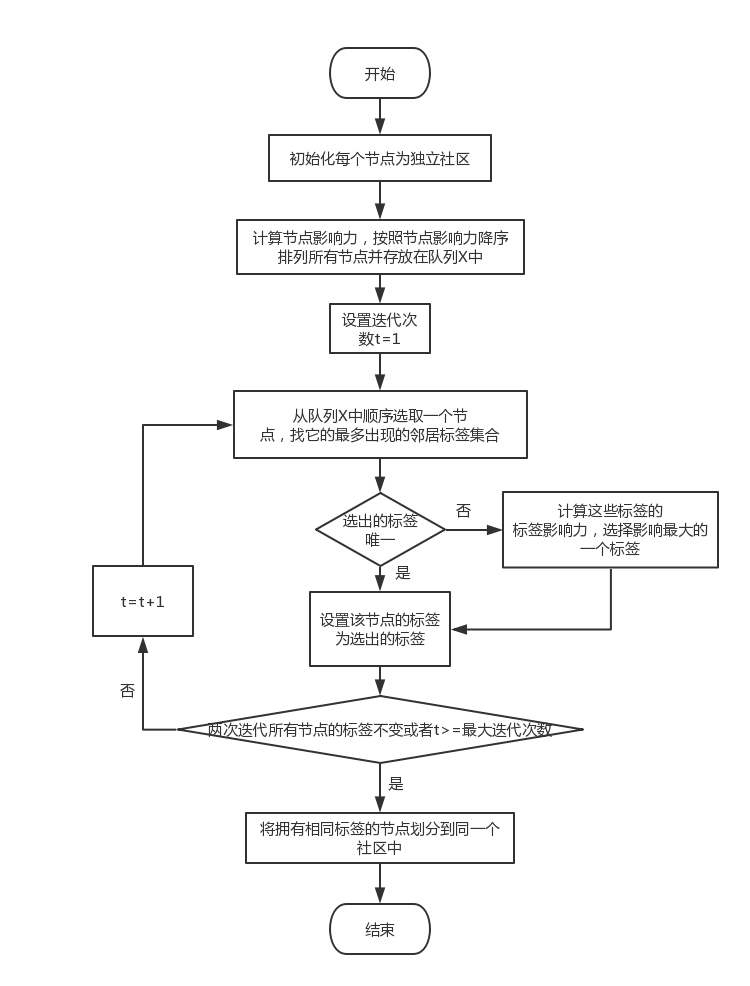
\includegraphics[width=1\textwidth]{figures/cdabslp}
  \caption{CDABSLP算法流程图}\label{fig:cdabslp}
 \end{figure}

下面结合一个实例来对CDABSLP算法的执行步骤进行详细说明,如图\ref{fig:CDABSLPshili}中所示。

\begin{figure}
  \centering
  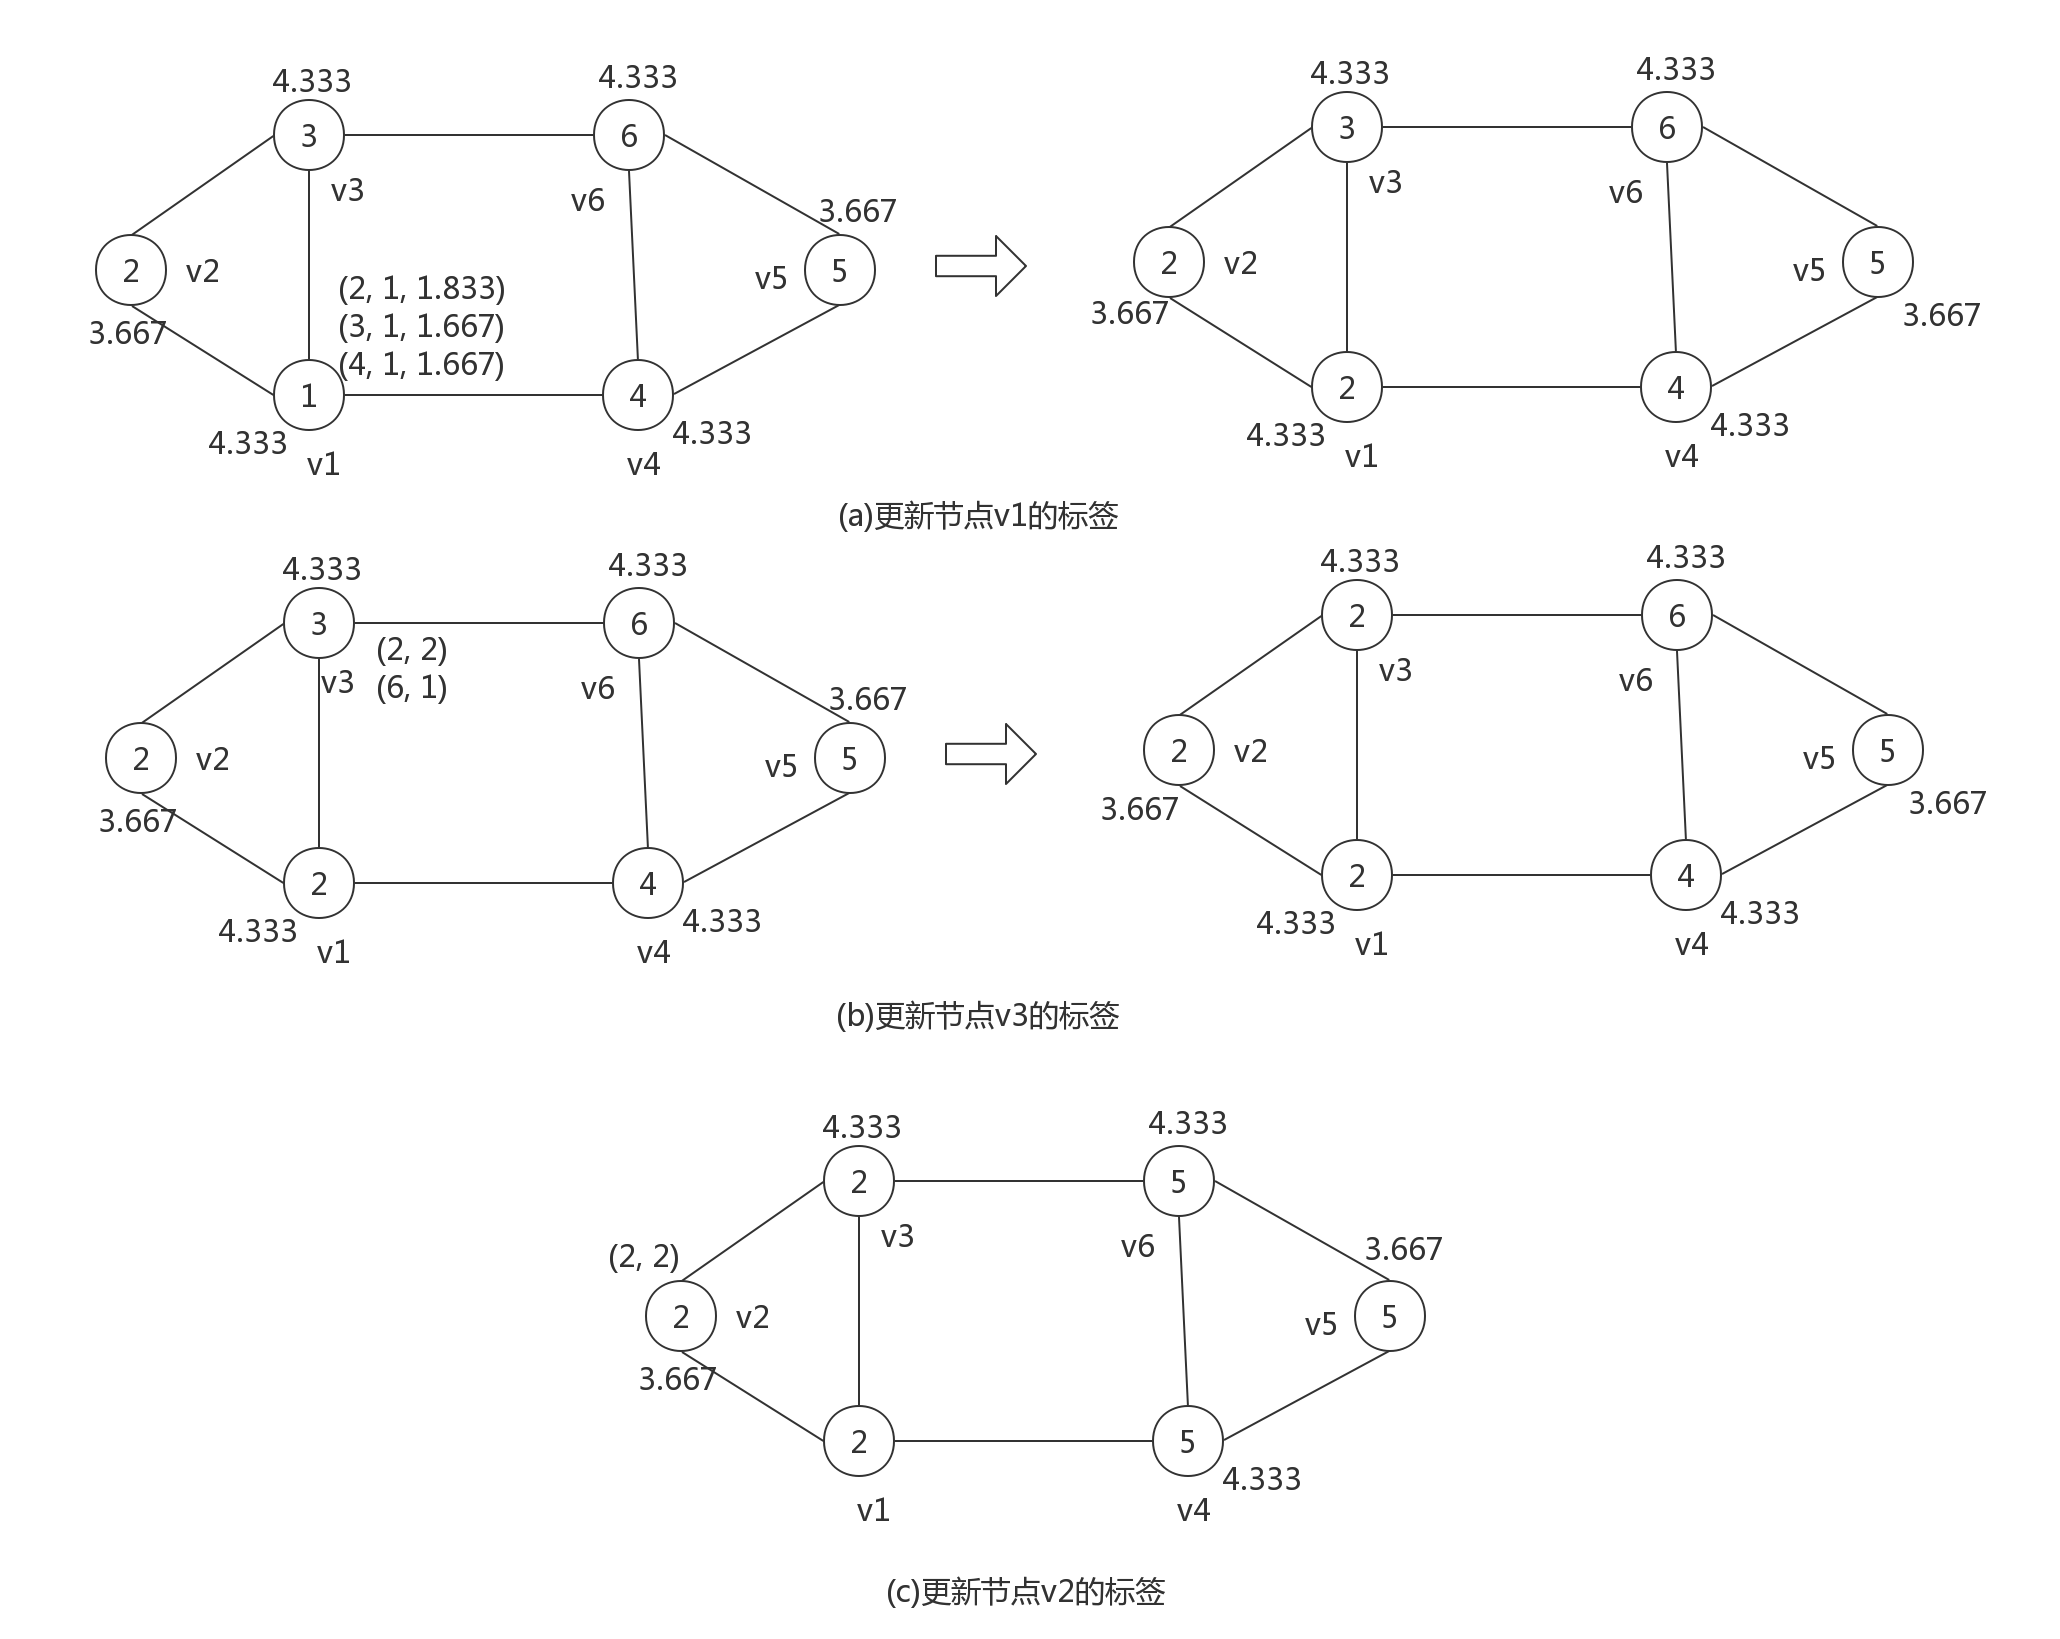
\includegraphics[width=0.75\textwidth]{figures/CDABSLPshili}
  \caption{CDABSLP算法标签传播过程示意图}\label{fig:CDABSLPshili}
 \end{figure}

\subsection{初始化阶段}

在算法的初始化阶段中:
\begin{enumerate}
  \item 每个节点被设置一个唯一的标签,即为其节点ID,在图\ref{fig:CDABSLPshili}中节点内的数字即为其初始化的标签,节点$\{ v_1,v_2,v_3,v_4,v_5,v_6 \} $的标签分别被初始化为$\{ 1,2,3,4,5,6 \} $;
  \item 对网络进行k-核分解,获取所有节点的k-核值$Ks(i)$,并在计算时,将中间过程中统计得出的每个节点的度保留下来以备下一步使用;
  \item 通过节点影响力公式\ref{eqn:NI}在初始化阶段计算每个节点的NI值,在图\ref{fig:CDABSLPshili}中每个节点外的浮点数值即代表其节点影响力大小,节点$\{ v_1,v_2,v_3,v_4,v_5,v_6 \} $的节点影响力分别为$\{ 4.333,3.667,4.333,4.333,3.667,4.333 \} $,此处小数点后仅保留了3位;
  \item 将所有节点以节点NI值大小降序排列,加入标签更新队列,NI值相同的节点,按照节点ID号升序排列,图\ref{fig:CDABSLPshili}所示的网络中,此排列即是按照$v_1-v_3-v_4-v_6-v_2-v_5$的顺序排列。
\end{enumerate}
CDABSLP算法初始化阶段具体可参考算法\ref{alg:CDABSLPchushihua}。

\begin{algorithm}[h]  
  \caption{CDABSLP算法初始化阶段}  
  \label{alg:CDABSLPchushihua} 
  \begin{algorithmic}[1]  
    \Require  
      社交网络$G=(V,E)$,节点影响力可调参数$\alpha$;  
    \Ensure  
      所有节点的影响力,标签更新队列;  
    \State 为网络G中每个节点设置一个唯一的标签,通常为其节点ID;  
    \State 对网络G进行k-核分解,获取所有节点的k-核值$Ks(i)$; 
    \State 通过节点影响力公式计算每个节点的节点影响力; 
    \State 将所有节点以节点影响力大小的降序进行排列后加入标签更新队列,节点影响力相同的节点,按照节点ID号升序排列; 
  \end{algorithmic}  
\end{algorithm}  

\subsection{标签传播阶段}

在算法的标签传播阶段中:
\begin{enumerate}
  \item 依次在标签更新队列中取出节点,找出它最多出现的邻居标签集合,在图\ref{fig:CDABSLPshili}(a)中展示了首先取出了节点$v_1$,它的三个邻居节点的标签各不相同,因此邻居标签最多出现次数为1,邻居标签集合即为$\{ 2,3,4 \} $;
  \item 判断找出的邻居标签集合是否唯一,若唯一则直接标签更新,若不唯一则按照公式\ref{eqn:LI}计算所有邻居标签的LI值,选择LI值最大的标签进行更新,若依然存在多个,则直接保留原标签,不进行更新,可以看见在图\ref{fig:CDABSLPshili}(a)中节点$v_1$的右上角有括号标注的三组数据,分别代表着标签$\{ 2,3,4 \} $分别出现了1次,对节点$v_1$的影响力分别为$\{ 1.833,1.667,1.667 \} $,此处小数点后仅保留了3位,显然标签“2”具有最大的影响力,故将节点$v_1$的标签更新为“2”,而在图\ref{fig:CDABSLPshili}(b)中可见CDABSLP算法在更新节点$v_3$的时候,因为标签“2”出现了两次,标签“6”仅出现一次,故将其更新为“2”,同理可按序将$\{ v_4,v_6,v_2,v_5 \} $更新为标签$\{ 5,5,2,5 \} $;
  \item 不断迭代直至标签不再更改或者已经达到最多迭代次数,在图\ref{fig:CDABSLPshili}中没有进行下一轮迭代的例图,但是不难知道,此例中的网络已经达到了最终收敛的稳定状态,结果也是符合预期的正确划分结果。仅仅只用了一轮标签传播,就在图\ref{fig:CDABSLPshili}所示网络中获得了稳定的划分状态,可见CDABSLP算法的输出结果是稳定而准确的。
\end{enumerate}
CDABSLP算法标签传播阶段具体可参考算法\ref{alg:CDABSLPlpa}。

\begin{algorithm}[h]  
  \caption{CDABSLP算法标签传播阶段}  
  \label{alg:CDABSLPlpa} 
  \begin{algorithmic}[1]  
    \Require  
      所有节点的影响力,标签更新队列,最大允许迭代轮数$maxIter$;  
    \Ensure  
      标签传播结果;  
    \State 迭代次数$iter=1$;  
    \Repeat  
      \State 在标签更新队列的队头取出节点$i$,找出它最多出现的邻居标签的集合$A = \{ l_1,l_2,...,l_m \} $;
      \If{$m==1$}  
        $//$找到的标签唯一
        \State 为节点$i$更新标签;  
      \Else  
        $//$找到的标签不唯一
        \State $max = 0$;
        \State $maxl = 0$;
        \For{each $l \in A$ }  
        $//$选择对节点$i$影响力最大的标签
          \State 计算$LI(i,l)$; 
          \If {$LI(i,l) > max$} 
            \State $max = LI(i,l)$;
            \State $maxl = l$;
          \EndIf 
          \State 将节点$i$标签更新为$maxl$;  
        \EndFor    
      \EndIf
      \State $iter = iter + 1$;  
    \Until{$iter > maxIter$ \textbf{or} 标签不再改变}
  \end{algorithmic}  
\end{algorithm}  

\section{算法时间复杂度分析}

CDABSLP算法的时间复杂度情况如下:

\begin{itemize}
  \item 所有节点初始化标签所花费的时间为$O(N)$;
  \item 所有节点影响力的计算所花费的时间为$O(M)$;
  \item 节点按照影响力大小降序排列所花费的时间为$O(N \cdot log(N))$;
  \item 标签迭代中的普通标签计算所花费的时间为$t \cdot O(M)$;
  \item 标签迭代中若遇到多个最大标签时,计算标签影响力所花费的时间为$t \cdot O(M)$;
  \item 社区划分过程所花费的时间为$O(N)$;
\end{itemize}

综上,CDABSLP算法的整体时间复杂度为:$2 \cdot O(N)+(2t+1) \cdot O(M)+O(N \cdot log(N))$;其中N,M,t分别表示节点总数、边的总数以及标签传播过程迭代次数,通常迭代次数不会很多,即相对于社交网络中N和M的大小,t一般仅是一个常数。可见CDABSLP算法在时间复杂度上虽然相较于原始LPA算法的线性复杂度有所增加,但是依然保持着很高的执行效率。

\section{验证实验}

本小节将为本章提出的CDABSLP算法进行实验验证。首先介绍实验的软硬件环境和采用的数据集,然后对算法的评价指标进行简单阐述,最后是相关对比实验的结果展示与分析,将CDABSLP算法与常用基准算法LPA算法和CNM算法\cite{Clauset2004Finding}进行对比,并与另一个基于LPA的改进算法KBLPA算法\cite{邓观明2016基于混合的}进行对比。考虑到LPA算法和KBLPA算法的实验结果不稳定,下面展示的实验结果均为多次实验的平均值。

\subsection{实验环境}

本章实现的CDABSLP算法所使用的机器配置如表\ref{tab:tab3-1}所示。CDABSLP算法使用Python语言编程实现,均基于Python的复杂网络相关软件包Networkx,使用Anaconda来对软件包进行管理和部署,具体配置如表\ref{tab:tab3-2}所示。

\begin{table}
  \centering
  \caption{计算机硬件配置} \label{tab:tab3-1}
  \begin{tabular*}{0.9\textwidth}{@{\extracolsep{\fill}}cccc}
  \toprule
    处理器			&2.2GHz 双核 Intel Core i7 \\
    内存容量			&8 GB 1600 MHz DDR3 \\
    硬盘容量			&128GB 固态硬盘 \\
  \bottomrule
  \end{tabular*}
% \end{table}

% \begin{table}
%   \centering
  \caption{计算机软件配置} \label{tab:tab3-2}
  \begin{tabular*}{0.9\textwidth}{@{\extracolsep{\fill}}cccc}
  \toprule
    操作系统			&macOS Sierra 10.12.6\\
    Anaconda版本  &conda 4.3.30 \\
    Networkx版本	&2.1 \\
    Python版本    &2.7.14\\
    Matplotlib版本  &2.0.2\\
    Numpy版本     &1.13.1\\
  \bottomrule
  \end{tabular*}
\end{table}

\subsection{数据集}

在本章的实验中,将分别采用真实网络中的数据集和LFR基准网络生成人工数据集来对CDABSLP算法的实验效果进行验证。
% 选用5个不同的真实数据集和LFR基准网络人工生成数据集进行实验验证本章所提算法的有效性。 

(1)真实数据集

在真实数据集中,本章实验选取了5个经典的数据集,包括Zachary Karate Club、American College Football、Dolphin Social Network等5个数据集。下面对这5个数据集进行简单介绍。

\begin{itemize}
  \item Zachary Karate Club数据集\cite{Zachary1977An}描绘的是美国一个大学空手道俱乐部34个成员彼此之间的社交网络,来自Zachary等人近3年的观察;因为其中主管和教练之间的矛盾,导致形成了两个小团体,即两个社区;在下文中将此数据集简记为N1。
  \item Dolphin Social Network数据集\cite{Lusseau2004Identifying}描绘的是新西兰一海湾居住的62只宽吻海豚彼此之间的社交网络,来自Lusseau等人长达7年的观察;在下文中将此数据集简记为N2。
  \item Pol Books数据集\cite{Polbooks}描绘的是根据在亚马逊上销售的政治相关书籍建立起来的政治派系网络,由Krebs等人通过人工分析而得,数据集中有自由派、中间派和保守派三个政治派系,即三个社区;在下文中将此数据集简记为N3。
  \item American College Football数据集\cite{football}描绘的是美国大学橄榄球比赛对阵情况,按照地区的不同,将各代表队分成了12个赛区,即12个社区;在下文中将此数据集简记为N4。
  \item Email数据集\cite{snapnets}描绘的是西班牙一大学里导师与研究生之间的邮件交互关系,由Guimer等人人工采集而得,该数据集并没有设定社区划分标准结果;在下文中将此数据集简记为N5。
\end{itemize}

真实数据集中的具体信息可参考表\ref{tab:tab3-3}。

% 在5个常用的真实网络数据集上进行实验验证本章算法的有效性,这5个真实网络数据集包括Karate、Dolphins 和 Football 等,各个数据集的详细信息如表\ref{tab:tab3-3}所示;

% N1:Karate是 Zachary 空手道俱乐部成员关系网络,网络中的所有节点对应各个成员,边表示两个端点对应的成员是好朋友。网络包含 34 个节点,78 条边和两个社区。 

% N2:Dolphins是 Lusseau 等人对栖息在新西兰 Doubtful Sound 峡湾的一个宽吻海豚群体进行长达 7 年的观察所构造出的海豚关系网,该群体包含 2 个家族共 62 只宽吻海豚。由这个群里的所有成员及它们间的接触关系构成一个包含62 个节点,159 条边和两个社区的网络。

% N3:Pol Books是从 Amazon 的图书销售记录抽象得到的网络数据集,分析了 105 本与美国政治相关的书和它们的 441 条共同销售关系,依据亚马逊上对图书的观点和评价情况,将这些书分为“自由派”、“中间派”和“保守派”三个类。因此,此数据集包含 105 个节点,441 条边和三个社区。

% N4:Football是分析美国高校橄榄球比赛对阵表得到的数据集。共有 115所高校派出代表队参赛,共进行了 616 场比赛,按各代表队地区的不同将这个包含 115 个节点 616 条边的网络分为 12 个社区。 

% N5:Email是由 Guimer 等人收集公布的,包含位于西班牙加泰罗尼亚自治区的罗维拉-威尔吉利大学(简称 URV)的教师和研究生之间的邮件往来关系。两个用户或者说两个邮箱地址如果互相发送过邮件,就构成一条边。网络包含 1133 个节点和 5451 条边。

\begin{table}
  \centering
  \caption{真实网络数据集} \label{tab:tab3-3}
  \begin{tabular*}{0.9\textwidth}{@{\extracolsep{\fill}}ccccc}
  \toprule
    数据集名称		&节点数   &边数   &社区数  &本文简称\\
  \midrule
    Zachary Karate Club  &34 &78 &2 &N1\\
    Dolphin Social Network	&62 &159  &2 &N2\\
    Pol Books  &105  &441  &3 &N3\\
    American College Football  &115  &616  &12 &N4\\
    Email     &1133 &5451 &- &N5\\
  \bottomrule
  \end{tabular*}
\end{table}

(2)LFR基准网络

在人工生成的基准网络之中,目前来说使用较为普遍的是GN基准网络\cite{2002Community}和LFR基准网络\cite{LFR}。早期的社区发现研究在进行实验分析时主要采用GN基准网络,但是无论如何调节设置参数z,GN基准网络生成的网络始终只有128个节点,这样的网络结构比较简单,因此也就缺少了很多真实社交网络中应有的特征。

而相对于GN基准网络,LFR基准网络深刻考虑到了真实社交网络中的“无标度”特征,可以自由对节点的度以及社区的大小等网络性质进行参数上的设置。因此,LFR基准网络已经成为当前最为流行的人工模拟数据集。在生成LFR人工数据集时需要设置的主要参数和它们的含义可参考表\ref{tab:tab3-4}。
% LFR基准网络是目前在社区发现领域使用最多的人工数据集之一。通过调整网络生成参数可以产生用户需要的不同的人工数据集,LFR 基准网络的主要生成参数及其含义如表\ref{tab:tab3-4}所示。

\begin{table}
  \centering
  \caption{LFR人工基准网络生成参数及其含义} \label{tab:tab3-4}
  \begin{tabular*}{0.9\textwidth}{@{\extracolsep{\fill}}cccc}
  \toprule
    参数		&含义\\
  \midrule
    N  &节点的个数\\
    avgk	&节点的平均度\\ 
    maxk  &节点的最大度\\
    minc  &最小社区包含的节点个数\\
    maxc  &最大社区包含的节点个数\\
    mu    &混合参数\\
    on    &重叠节点的个数\\
    om    &重叠节点最多可属于的社区个数\\
  \bottomrule
  \end{tabular*}
\end{table}

在表\ref{tab:tab3-4}中列出的所有参数里,需要进一步解释的是混合参数$mu$,$ mu \in [0,1]$。该参数表示的是社区内部节点与社区外部节点之间存在边的概率。在LFR人工数据集上进行社区发现的难度与$mu$参数值的大小成正比。$mu$越小,表明社区发现的难度越小,而$mu$越大,表明社区发现的难度越大。

为了能充分验证CDABSLP算法的效果,利用LFR基准网络生成程序生成了6组非重叠社区的人工数据集,将其编号分别记为$L1\sim L6$。具体参数设置可参考表\ref{tab:tab3-5}。其中所有生成网络中的maxk均设置为500,每组数据中按照mu参数从0.1到0.9分别生成9个数据集,而在非重叠社区数据集的生成过程中,on和om选择默认值0和1即可。
% 在 LFR 模型众多的生成参数中,混合参数$ mu \in [0,1]$是非常重要的一个参数,mu 越小,说明连接社区之间的边越少,社区之间越“分离”,社区划分的难度随着 mu 的增长而增大。on 和 om 两个参数用于生成具有重叠社区的数据集,生成具有非重叠社区结构的数据集时,只需将 on 设置为 0,om 设置为 1 即可。 
% 生成六组具有非重叠社区结构的 LFR 基准网络数据集,所有的网络共享的相同参数是 maxk = 500、on = 0 和 om = 1。每组包含九个 mu 值不同的数据集,分别为 0.1 到 0.9,每组中的九个数据集共享参数 N、avgk、minc 和 maxc。其他参数都取默认值。表\ref{tab:tab3-5}展示了这六组网络详细的生成参数情况。 

\begin{table}
  \centering
  \caption{LFR基准网络在非重叠社区数据集上的生成参数} \label{tab:tab3-5}
  \begin{tabular*}{0.9\textwidth}{@{\extracolsep{\fill}}ccccc}
  \toprule
    编号		&N  &avgk  &minc &maxc \\
  \midrule
    L1  &10000  &100  &10 &500 \\
    L2  &10000  &100  &20 &100 \\
    L3  &50000  &100  &10 &500 \\
    L4  &50000  &100  &20 &100 \\
    L5  &10000  &200  &10 &500 \\
    L6  &10000  &200  &20 &100 \\
  \bottomrule
  \end{tabular*}
\end{table}
% \begin{table}
%   \centering
%   \caption{LFR基准网络在非重叠社区数据集上的生成参数} \label{tab:tab3-5}
%   \begin{tabular*}{0.9\textwidth}{@{\extracolsep{\fill}}ccccccc}
%   \toprule
%     编号		&N  &avgk &maxk &minc &maxc &mu\\
%   \midrule
%     L1  &10000  &100 &500 &10 &500 &$0.1\sim 0.9$\\
%     L2  &10000  &100 &500 &20 &100 &$0.1\sim 0.9$\\
%     L3  &50000  &100 &500 &10 &500 &$0.1\sim 0.9$\\
%     L4  &50000  &100 &500 &20 &100 &$0.1\sim 0.9$\\
%     L5  &10000  &200 &500 &10 &500 &$0.1\sim 0.9$\\
%     L6  &10000  &200 &500 &20 &100 &$0.1\sim 0.9$\\
%   \bottomrule
%   \end{tabular*}
% \end{table}

\subsection{评价指标}

随着社区发现算法的不断提出,针对如何评判社区发现结果的优劣这一问题,研究人员们也同样提出了很多评价指标。本章将采用模块度、标准化互信息(NMI)和F-measure值。下面介绍这三个评价指标:
% 迄今为止,出现了各种各样的社区发现算法,如何评价不同的的发现算法的好坏是一个非常重要的问题。为此,学者们提出了多种社区结构评价指标用来评价网络社区划分质量,其中比较有代表性的有模块度、NMI等。下面介绍这些指标。

(1)模块度

模块度\cite{2002Community}是Newman等人在提出GN算法之后,用以解决当时的社区发现算法无法很好地衡量社区划分结果质量的问题,专门提出的用以评价社区划分结果的评价指标。模块度通过对比划分后的网络与随机网络在相同社区划分的情况下的社区内的连接密度来衡量社区划分的质量,其中的随机网络是与原始网络拥有同样节点度序列的随机网络。通常情况下将模块度即为Q,其具体计算方式可参考公式\ref{eqn:modular}。
% 模块度是目前学者们最常用和经典的网络社区结构评价指标,它最初是被Newman等人于2004年提出来的\cite{2002Community}。其通过比较现有网络和基准网络在相同社区划分下的连接密度差来衡量网络社区的优劣,其中基准网络是由原网络具有相同度序列的随机网络。模块度计算方式详见公式\ref{eqn:modular}。

\begin{equation}
  \label{eqn:modular}
  Q=\frac{1}{2m}\sum_{i,j}\left [ A_{ij}-\frac{k_ik_j}{2m} \right ]\delta (c_i, c_j)  
\end{equation}

其中,社交网络以邻接矩阵矩阵A表示,m代表着边的总数,$k_i$代表节点i的度数,$c_i$代表节点i被划分而得的社区编号。若$i=j$,则$\delta(c_i,c_j)=1$,反之$\delta(c_i,c_j)=0$
% 其中,A 表示网络中的邻接矩阵, m 表示网络中边的总数,$k_i$和$k_j$表示节点 i 和 j 的度数,表示节点 i 和 j 的度数,$c_i$和$c_j$表示节点 i 和 j 所属的社区。如果$i=j,\delta(c_i,c_j)=1$,反之$\delta(c_i,c_j)=0$

(2)标准化互信息(NMI)

模块度指标在对社区划分进行评判的时候,无需知道社区的标准划分结果,常用于没有标准划分的真实网络数据集之中,但是对于一些已经知道标准划分的数据集来说,文献\cite{Peng2014Weighting}中采用的标准化互信息(Normalized Mutual Information,一般缩写为NMI,中文翻译上也有学者将其译作“归一化互信息”)可以作为一个更为精确的衡量指标。NMI指数通常是被用于聚类之中,用于衡量两个聚类结果之间的相似程度,被引入社区发现领域后,已然成为了一个重要的社区划分结果优劣的衡量指标。它基本上能够较为客观地分析一个社区划分与标准划分相比而言的差距,能很好地评判划分的准确性。NMI指数的取值范围是0到1,数值越高表示社区发现结果越准确。它的计算方法可参考公式\ref{eqn:nmi}。
% 随着在线社交网络的发展,人们发现在线社交网络的很多数据中存在着暗示各个节点的社区属性信息。例如,在人人网的学校信息便揭示了网络节点中属于同一学校的社区结构,Facebook中的兴趣信息同样表征了具有相同兴趣的虚拟用户群体。这些数据在为社区发现问题提供了丰富的信息的同时,也在一定程度上为虚拟社区结构优劣的评判提供了标准答案。针对这种预先拥有一定虚拟社区结构信息的情况下,文献\cite{Peng2014Weighting}中提到了Normalized Mutual Information(NMI),利用信息化熵来衡量算法划分的社区结构和预先已知的社区结构之间的差异。NMI是基于混合矩阵(Confusion Matrix)N来计算的数字指标。NMI计算方式详见公式\ref{eqn:nmi}。

\begin{equation}
  \label{eqn:nmi}
  NMI=\frac{ -2 \sum_{i,j} N_{ij}  ln{\frac{N_{ij}}{N_iN_j}} } {\sum_{i}N_iln{\frac{N_i}{n}}+\sum_{j}N_jln{\frac{N_j}{n}}}
\end{equation}

其中,n代表网络中节点的总数,$N_i$表示社区i中的节点个数,$N_{ij}$代表的是社区i和社区j之间有连接的节点的总数。
% 使用该数字指标,可以衡量划分出来的社区结构与已知的网络社区结构的差异程度值,该值越大,则表明获得的社区结构划分越好,当该值达到最大化值1时,说明算法发现的社区结构与已知社区结构完全已知,效果最好。

\begin{figure}
 \centering
 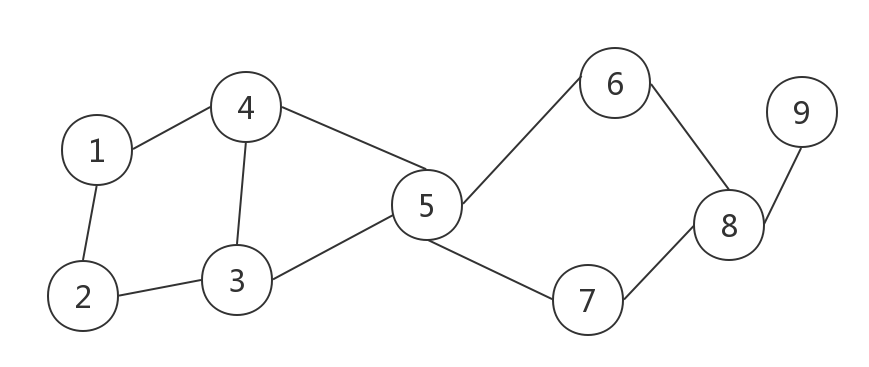
\includegraphics[width=0.75\textwidth]{figures/fig5-1}
 \caption{NMI网络示例图}\label{fig:fig5-1}
\end{figure}

% 下面以图\ref{fig:fig5-1}为例来说明计算NMI的过程。假设已知的最佳社区结构划分为集合{1,2,3,4}和{5,6,7,8},相应的社区划分向量表示为a = (1,1,1,1,2,3,3,3,3),再假设某算法获得的社区划分结构可以用向量表示为b = (3,3,3,3,2,1,1,1,1)来表示。根据已知的社区划分向量,可以构造混合矩阵\ref{eqn:n}。

% \begin{equation}
%   \label{eqn:n}
%   N=\begin{bmatrix}
%     0 & 0 &4 \\ 
%     0 & 1 & 0\\ 
%     4 & 0 & 0
%     \end{bmatrix}
% \end{equation}

% 根据上式计算可知,该划分的NMI值为1。

(3)PWF

成对F-measure值即Pairwise F-measure值,下文将采用缩写形式PWF来指导该指标。其计算方法具体可参考公式\ref{eqn:pwf}。
% 成对 F-measure(Pairwise F-measure,PWF)是成对准确率(Pairwise Precision,PWP)和成对召回率(Pairwise Recall,PWR)的调和,其计算如公式\ref{eqn:pwf}所示。

\begin{equation}
  \label{eqn:pwf}
  PWF=\frac{2\cdot PWP\cdot PWR}{PWP+PWR}
\end{equation}

其中PWP代表的是成对准确率(Pairwise Precision),PWP的计算公式具体可参考公式\ref{eqn:pwp};而PWR代表的是成对召回率(Pairwise Recall),PWR的计算公式具体可参考公式\ref{eqn:pwr}。
% 成对准确率(PWP)和成对召回率(PWR)的计算公式分别为公式\ref{eqn:pwp}和公式\ref{eqn:pwr}。

\begin{equation}
  \label{eqn:pwp}
  PWP=\frac{ \left | S \cap T \right |}{ \left | S \right |}
\end{equation}

\begin{equation}
  \label{eqn:pwr}
  PWR=\frac{ \left | S \cap T \right |}{ \left | T \right |}
\end{equation}

其中,T代表着在数据集的正确社区发现结果中属于相同社区的节点对集合,而S代表在经过社区发现算法之后网络的社区划分结果中属于相同社区的节点对集合,$S \cap T $ 即是两者的交集,表示划分正确的节点集合,而对集合S两端加绝对值$\left | S \right |$,表示集合S中的元素个数。

与NMI类似,PWF值的大小同样是与社区划分质量的优劣成正比。
% T 表示在真实的社区划分结果中,在同一个社区内的节点对集合;S 表示在测试算法得到的社区划分结果中在同一个社区内的节点对集合;$\left | S \cap T \right |$ 表示在真实的社区划分结果和测试划分结果中都在同一个社区内的节点对集合。PWF 的取值范围是 $0 \sim 1$,PWF 越大,说明社区划分的准确率越高。

\subsection{实验结果及分析}

(1)真实网络数据上的实验

本章首先对上文介绍的五个真实数据集进行对比实验,采用的评价指标为模块度和NMI。所有数据集最终得到的模块度Q值可参见表{tab:tab3-6},而由于数据集N5并没有标准网络划分结果,因此无法对其使用NMI评价指标,故$N1 \sim N4$数据集最终得到的NMI值可参见表\ref{tab:tab3-7}。考虑到LPA算法和KBLPA算法实验结果的不稳定性,为了更好地凸显其不稳定的结果,它们的模块度与NMI值将会以均值±最大偏差的形式来展示。
% 在数据集中介绍的5个真实网络数据集经常出现在社区发现的文献中,使用模块度 Q 和标准化互信息 NMI 作为前四个数据集上实验结果的评价指标,而另外一个数据集上仅使用模块度 Q 作为评价指标。表\ref{tab:tab3-6}和表\ref{tab:tab3-7}给出了四种对比算法在5个真实网络数据集上的实验结果,由于 N5 网络的真实社区结构未知,所以在表 3-8 中仅给出了前四个网络上实验结果的 NMI 值。每个数据集上得到的最优的 Q 和 NMI 值用粗体表示,LPA算法和 CDABSLP 算法得到结果的 Q 和 NMI 以平均值±最大偏差的形式表示。

\begin{table}
  \centering
  \caption{真实网络数据集实验的模块度大小对比} \label{tab:tab3-6}
  \begin{tabular*}{0.9\textwidth}{@{\extracolsep{\fill}}ccccc}
  \toprule
    编号		&LPA  &CNM &KBLPA &CDABSLP \\
  \midrule
    N1  &$0.286 \pm 0.28$  &0.355 &$0.083 \pm 0.22$ &0.433 \\
    N2  &$0.455 \pm 0.18$  &0.316 &$0.499 \pm 0.11$ &0.531 \\
    N3  &$0.479 \pm 0.14$  &0.275 &$0.459 \pm 0.08$ &0.507 \\
    N4  &$0.572 \pm 0.13$  &0.547 &$0.583 \pm 0.08$ &0.592 \\
    N5  &$0.370 \pm 0.26$  &0.425 &$0.293 \pm 0.23$ &0.437 \\
  \bottomrule
  \end{tabular*}
\end{table}

\begin{table}
  \centering
  \caption{真实网络数据集实验的NMI大小对比} \label{tab:tab3-7}
  \begin{tabular*}{0.9\textwidth}{@{\extracolsep{\fill}}ccccc}
  \toprule
    编号		&LPA  &CNM &KBLPA &CDABSLP \\
  \midrule
    N1  &$0.573 \pm 0.48$  &0.445 &$0.183 \pm 0.33$ &1 \\
    N2  &$0.516 \pm 0.29$  &0.436 &$0.491 \pm 0.24$ &0.662 \\
    N3  &$0.564 \pm 0.17$  &0.245 &$0.534 \pm 0.11$ &0.676 \\
    N4  &$0.853 \pm 0.14$  &0.646 &$0.659 \pm 0.12$ &0.898 \\
  \bottomrule
  \end{tabular*}
\end{table}

从表\ref{tab:tab3-6}中不难看出,四个算法中,CDABSLP算法划分得到的社区计算出的模块度是最大的,且结果相对稳定,这表明了算法在社区划分质量和算法稳定性上均取得了不错的效果。其中KBLPA算法在这几个数据集上的表现并未比LPA算法优化多少,尽管在稳定性上比LPA算法强了一些,但是依然存在着结果不稳定的问题,且整体划分质量反而有所下降;而CNM算法则介于LPA算法、KBLPA算法和CDABSLP算法之间,相对比较中庸,虽然划分质量一般,但是贵在稳定。

在表\ref{tab:tab3-7}中反应的NMI结果来看,CDABSLP算法的优势将显得更加明显。四个数据集上CDABSLP算法均取得了远大于CNM算法的NMI值,而在稳定性上,CDABSLP算法又远胜于另外两种基于标签传播的算法。

综上所述,CDABSLP算法在真实网络数据集上具有较好的稳定性,且发现结果质量良好。
% 从表\ref{tab:tab3-6}和表\ref{tab:tab3-7}可以看出,CDABSLP 算法得到社区结构的模块度 Q 比其他三种算法都高。同时,CDABSLP 算法在前四个网络上得到的社区结构的 NMI 值也是最优的。KBLPA 算法的稳定性优于 LPA 算法,但是 KBLPA 算法在几乎所有网络上得到社区结构的 Q 和 NMI都没有 LPA 算法好。实验结果表明,CDABSLP 算法能够得到比其他三种算法更好更稳定的社区检测结果。

(2)LFR人工基准网络上的实验

图\ref{fig:S1deNMIhePWF} $\sim$ \ref{fig:S6deNMIhePWF}分别是四种算法在六组非重叠 LFR 基准网络数据集
(S1$\sim$S6)上实验结果的 NMI 和 PWF 指标的对比图。横轴代表混合参数 mu,取
值从 0.1 到 0.9;左侧六幅图的纵轴代表社区划分结果的 NMI 值,右侧六幅图的
纵轴表示实验结果的 PWF 值。

\begin{figure}
  \centering
  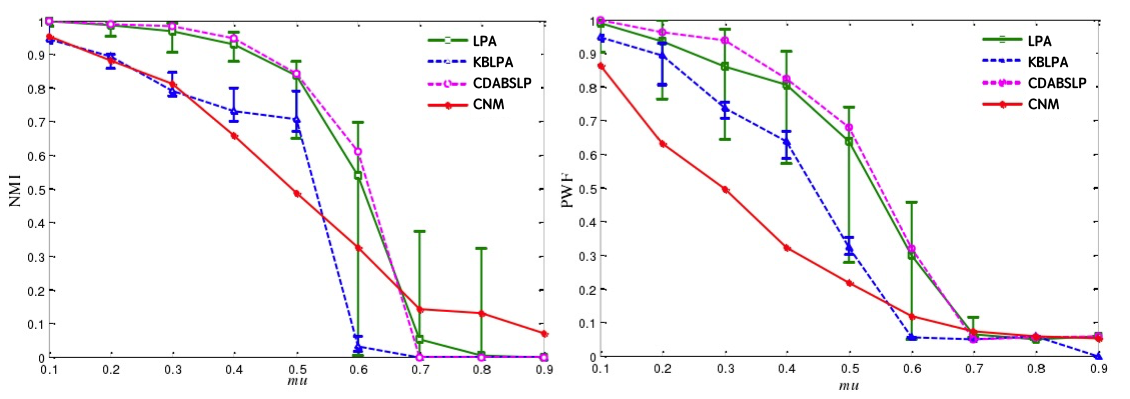
\includegraphics[width=0.75\textwidth]{figures/S1deNMIhePWF}
  \caption{在S1网络上的实验结果的NMI和PWF比较}\label{fig:S1deNMIhePWF}

  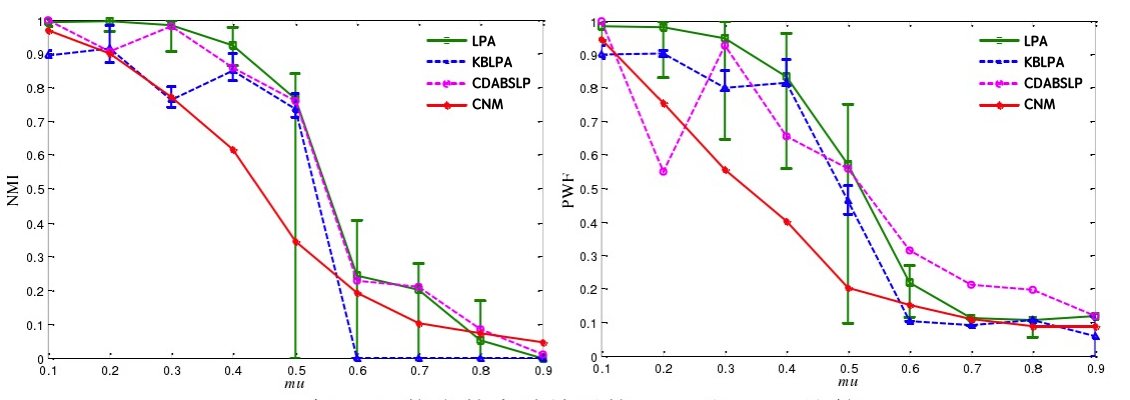
\includegraphics[width=0.75\textwidth]{figures/S2deNMIhePWF}
  \caption{在S2网络上的实验结果的NMI和PWF比较}\label{fig:S2deNMIhePWF}

  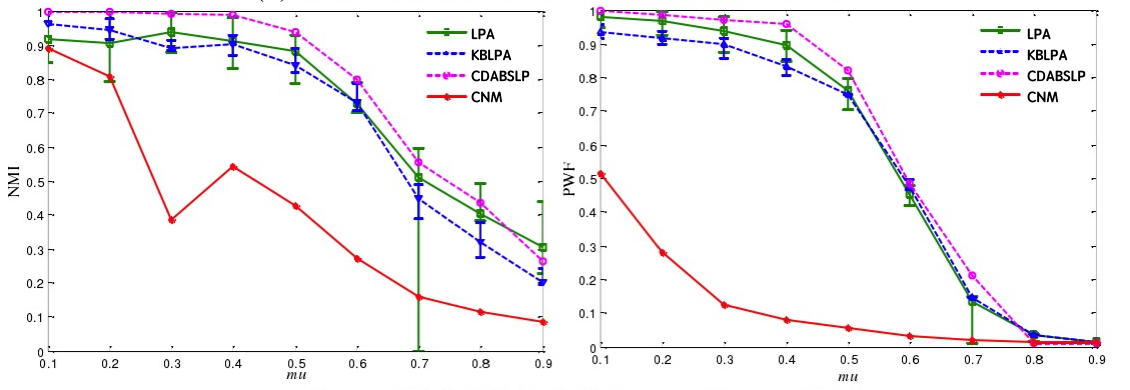
\includegraphics[width=0.75\textwidth]{figures/S3deNMIhePWF}
  \caption{在S3网络上的实验结果的NMI和PWF比较}\label{fig:S3deNMIhePWF}

  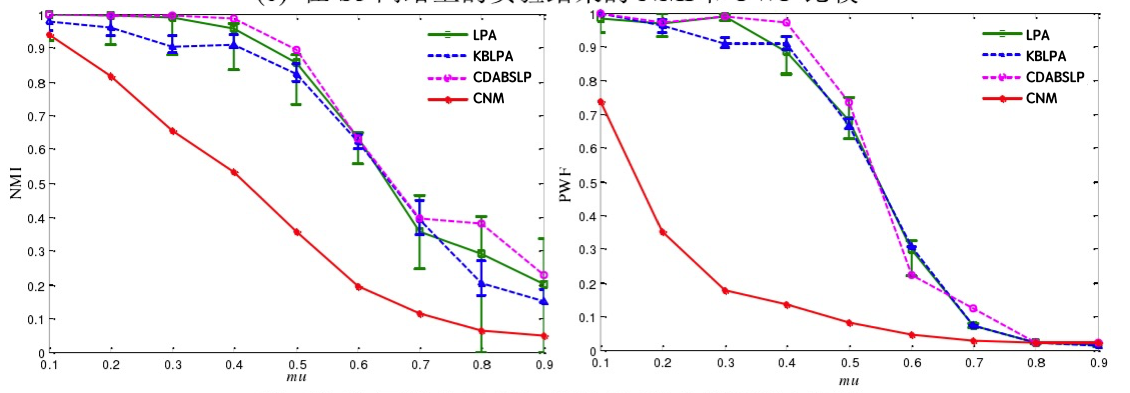
\includegraphics[width=0.75\textwidth]{figures/S4deNMIhePWF}
  \caption{在S4网络上的实验结果的NMI和PWF比较}\label{fig:S4deNMIhePWF}
\end{figure}

\begin{figure}
  \centering
  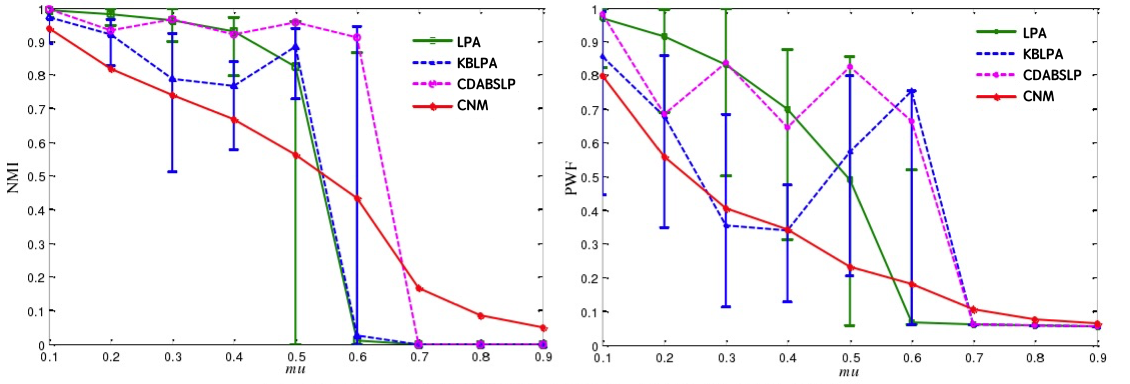
\includegraphics[width=0.75\textwidth]{figures/S5deNMIhePWF}
  \caption{在S5网络上的实验结果的NMI和PWF比较}\label{fig:S5deNMIhePWF}

  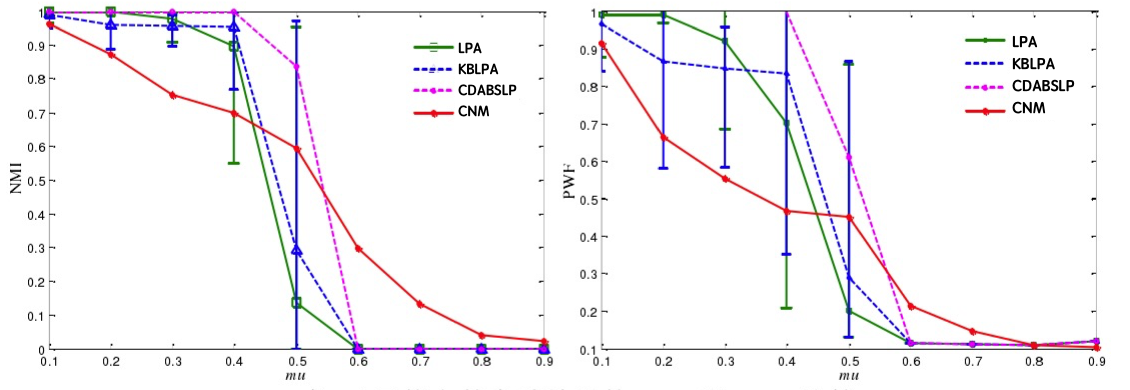
\includegraphics[width=0.75\textwidth]{figures/S6deNMIhePWF}
  \caption{在S6网络上的实验结果的NMI和PWF比较}\label{fig:S6deNMIhePWF}
\end{figure}

图\ref{fig:S1deNMIhePWF} $\sim$ \ref{fig:S6deNMIhePWF}中的 12 幅图可以看出,随着 mu 值的增大,网络的结构越来越复杂,
社区结构越来越不明显,四种算法得到的社区划分结果都随之变差,尤其是当
mu 大于 0.5 时,NMI 和 PWF 指标下降的更快。但是,整体来看,CDABSLP 算法
的效果优于其他三种算法。虽然 CDABSLP 算法并不是在所有情况下都能得到最优
的结果,但是它得到的结果是稳定的并且比较好的。从对比图中还能看出 LPA
算法得到结果的 NMI 和 PWF 的波动都很大;KBLPA 算法得到的结果是比较稳
定的,但是该算法检测得到的社区结构比 LPA 和 CDABSLP 算法都要差一些。在
所有这些 LFR 网络上,CNM 算法并不能检测到最优的社区结构,而且它得到的
社区的数目通常都比真实情况少。 



(3)可视化对比

将 CDABSLP 算法在 Dolphins 数据集上检测得到的社区结构和 Dolphins网络
真实的社区结构进行比较,如图\ref{fig:Dolphins}所示。

\begin{figure}
  \centering
  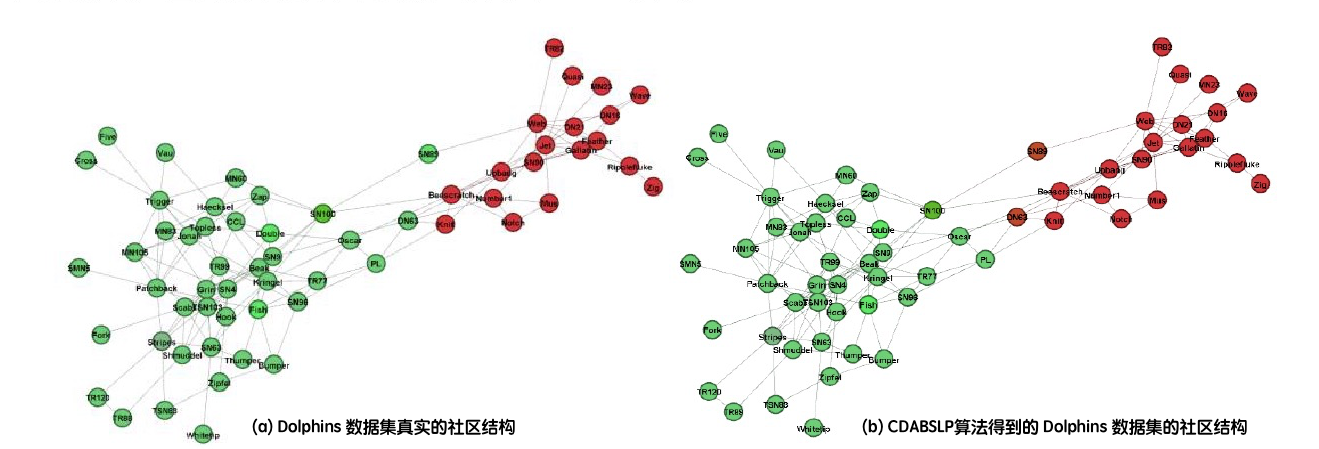
\includegraphics[width=0.75\textwidth]{figures/Dolphins}
  \caption{Dolphins 数据集的社区结构}\label{fig:Dolphins}
\end{figure}

图\ref{fig:Dolphins}(a)展示的是 Dolphins 网络真实的社区结构,节点不同的颜色表示不
同社区;图\ref{fig:Dolphins}(b)是 CDABSLP 在 Dolphins 网络上检测到的社区结构图。通过比
较这两幅图, CDABSLP 算法得到的结果中,节点 DN63 和 SN90 的划分与 Dolphins
真实的社区结构不同。从 Dolphins 网络的拓扑结构发现,节点 DN63 有两个邻接
点,它们分别属于两个不同的社区;节点 DN63 有五个邻接点, CDABSLP 算法将
DN63 划分到了它的多数邻接点所在的社区。Dolphins 网络的真实的社区结构的
模块度比 CDABSLP 算法得到的社区结构的模块度小,可以看出 CDABSLP 算法得到
的结果是合理的。

(4)参数选择实验

在 CDABSLP 算法中只有一个参数,即调节参数$\alpha$。为了分析参数对算法的影
响,设置不同的参数$\alpha$值,在人工网络数据集上运行 CDABSLP 算法,通过比较
结果的 NMI 分析参数对算法的影响。通过这种方法,能够发现参数$\alpha$取什么值
时能够得到最好的结果。

生成五个 LFR 基准数据集,参数 avgk 分别从 10 到 50,其他的生成参数相
同(N = 1000、maxk = 50、minc = 10、maxc = 50 和 mu = 0.1)。图\ref{fig:alpha}显示了
CDABSLP 算法在这些网络上的实验结果,横轴代表参数$\alpha$的不同取值,从 0 到 1,
纵轴代表 NMI 值。

\begin{figure}
  \centering
  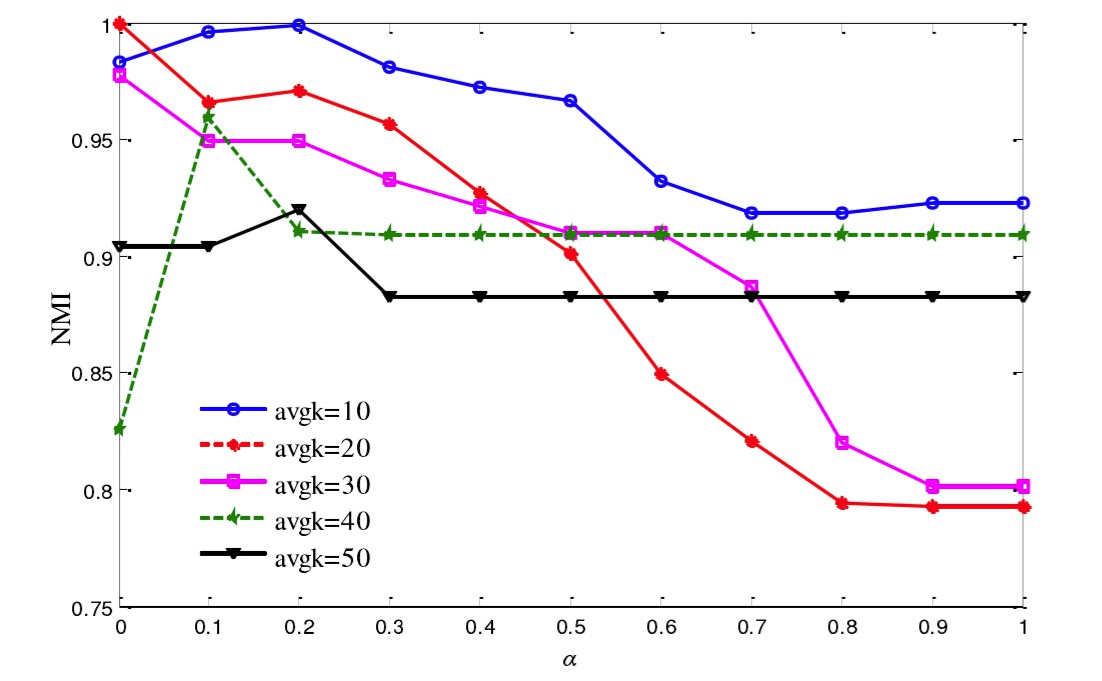
\includegraphics[width=0.75\textwidth]{figures/alpha}
  \caption{不同$\alpha$值对结果的影响}\label{fig:alpha}
\end{figure}

从图\ref{fig:alpha}中可以看出,参数$\alpha$取不同值的情况下,算法得到结果的 NMI 值
变化很大。但是,对于每个网络,都存在一个最优的$\alpha$值使得 CDABSLP 算法能够
得到 NMI 值最大的社区划分结果。此外,还能看出,在每个网络上得到的第一
个极大值基本就是该网络上的最优值。

(3)不同规模网络的实验对比

生成十个不同规模的 LFR 基准网络数据集来验证算法的时间效率。网络中
节点个数设置为从 1000 到 10000 的十个不同的网络,其他的生成参数相同,均为
avgk = 10、maxk = 50、minc = 10、maxc = 50 和 mu = 0.1。 
图\ref{fig:butongguimowangluobijiao}左侧显示了四种算法在十个不同规模网络上运行时间的比较,图 \ref{fig:butongguimowangluobijiao}右侧
是左侧图的放大图,只显示了 LPA、KBLPA 和 CDABSLP 三种算法。

\begin{figure}
  \centering
  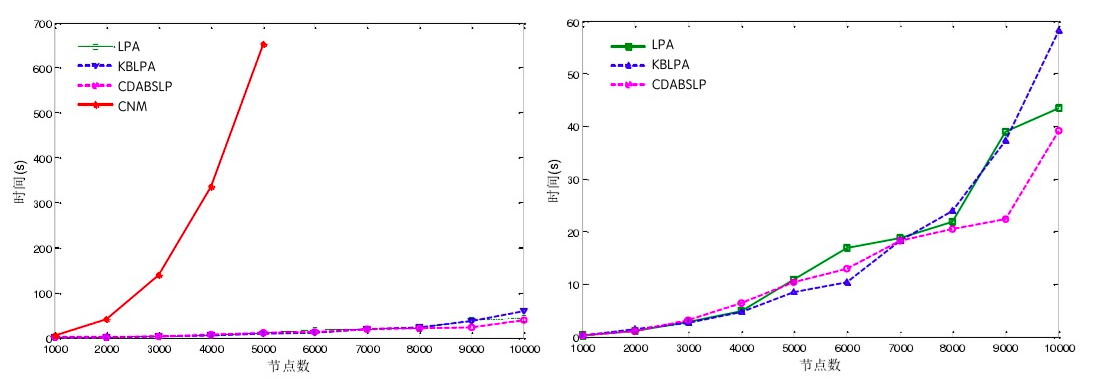
\includegraphics[width=0.75\textwidth]{figures/butongguimowangluobijiao}
  \caption{四种算法在不同规模网络上的效率比较}\label{fig:butongguimowangluobijiao}
\end{figure}

从图\ref{fig:butongguimowangluobijiao}可以看出,随着网络规模的增大,四种算法所用时间不断增加,其
中 CNM 算法所用时间是最长的,这是由于 CNM 算法迭代的次数远远多于其他
三种基于标签传播的算法的迭代次数。当网络规模大于 5000 时,由于计算机内
存限制 CNM 算法不能得到网络的社区结构。在图\ref{fig:butongguimowangluobijiao}右侧中,能更清楚的看到当
节点大于 7000 时,CDABSLP 算法所用时间比 LPA 算法少,说明 CDABSLP 算法比
LPA 算法更适合用于大规模复杂网络社区发现,这是因为 CDABSLP 算法的标签传
播迭代次数比 LPA 算法少,能够更快的趋于稳定。 


% \subsection{实验总结}

% CDABSLP算法从两个方面改善 LPA 算法不稳定的问题:首先,计算
% 网络中每个节点的节点影响值并按节点影响值降序排列作为节点标签更新的顺
% 序,取代传统 LPA 算法中节点更新顺序随机确定的方法;其次,在每次标签更
% 新迭代过程中,当传统的标签计算方法返回多个标签时,提出一种新的标签计算
% 公式,计算返回标签的影响强度,在返回的多个标签中重新选择一个影响强度最
% 大的标签作为该节点的新标签,以此替代传统 LPA 算法中随机选择一个标签的
% 方法。CDABSLP算法既保持了传统 LPA 算法的优点,还解决了 LPA 算法不稳定
% 的问题,该算法能够得到稳定的社区结构。大量实验结果表明CDABSLP算法的性
% 能优于目前一些代表性的社区发现算法。 

\section{本章小结}

本章主要介绍了一种基于稳定标签传播的非重叠社区发现算法,简称CDABSLP。在简单分析了原始LPA算法存在的缺陷之后,针对相应的缺陷逐一介绍其稳定性解决方案。算法在标签更新的时候采用异步更新的策略;然后提出了一种综合节点自身重要性以及邻居节点重要性的节点影响力模型,将节点更新顺序设为节点影响力的降序;最后在标签选择时出现多个最大标签的情况下,提出了一种标签影响力模型,在多个标签中,计算每个标签对当前节点的影响力,选取其中影响力最大的标签进行标签更新,当影响力最大的标签依然存在多个时,选择保留原标签不进行更改。通过真实网络以及人工网络中的验证实验,可知CDABSLP算法在具有良好的稳定性的同时兼具较高的运行效率,在多个评价指标之上社区发现准确率均有不错的表现。
